%!TEX TS-program = xelatex
\documentclass[notes,12pt, aspectratio=169]{beamer}

\usepackage{amsmath,amsfonts,amssymb,amsthm,mathtools}  % пакеты для математики
%\usepackage{minted}

\usepackage[english, russian]{babel} % выбор языка для документа
\usepackage[utf8]{inputenc} % задание utf8 кодировки исходного tex файла
\usepackage[X2,T2A]{fontenc}        % кодировка

\usepackage{fontspec}         % пакет для подгрузки шрифтов
\setmainfont{Helvetica}  % задаёт основной шрифт документа

% why do we need \newfontfamily:
% http://tex.stackexchange.com/questions/91507/
\newfontfamily{\cyrillicfonttt}{Helvetica}
\newfontfamily{\cyrillicfont}{Helvetica}
\newfontfamily{\cyrillicfontsf}{Helvetica}

\usepackage{unicode-math}     % пакет для установки математического шрифта
% \setmathfont{Neo Euler} % шрифт для математики

\usepackage{polyglossia}      % Пакет, который позволяет подгружать русские буквы
\setdefaultlanguage{russian}  % Основной язык документа
\setotherlanguage{english}    % Второстепенный язык документа

% Шрифт для кода
\setmonofont[Scale=0.85]{Monaco}
\usepackage{verbments}

\usepackage{pgfpages}
% These slides also contain speaker notes. You can print just the slides,
% just the notes, or both, depending on the setting below. Comment out the want
% you want.
%\setbeameroption{hide notes} % Only slide
%\setbeameroption{show only notes} % Only notes
%\setbeameroption{show notes on second screen=right} % Both

\usepackage{array}

\usepackage{tikz}
\usepackage{verbatim}
\setbeamertemplate{note page}{\pagecolor{yellow!5}\insertnote}
\usetikzlibrary{positioning}
\usetikzlibrary{snakes}
\usetikzlibrary{calc}
\usetikzlibrary{arrows}
\usetikzlibrary{decorations.markings}
\usetikzlibrary{shapes.misc}
\usetikzlibrary{matrix,shapes,arrows,fit,tikzmark}

\usepackage{hyperref}
\usepackage{lipsum}
\usepackage{multimedia}
\usepackage{multirow}
\usepackage{dcolumn}
\usepackage{bbm}
\newcolumntype{d}[0]{D{.}{.}{5}}

\usepackage{changepage}
\usepackage{appendixnumberbeamer}
\newcommand{\beginbackup}{
   \newcounter{framenumbervorappendix}
   \setcounter{framenumbervorappendix}{\value{framenumber}}
   \setbeamertemplate{footline}
   {
     \leavevmode%
     \hline
     box{%
       \begin{beamercolorbox}[wd=\paperwidth,ht=2.25ex,dp=1ex,right]{footlinecolor}%
%         \insertframenumber  \hspace*{2ex} 
       \end{beamercolorbox}}%
     \vskip0pt%
   }
 }
\newcommand{\backupend}{
   \addtocounter{framenumbervorappendix}{-\value{framenumber}}
   \addtocounter{framenumber}{\value{framenumbervorappendix}} 
}

% для имитации питоновского синтаксиса 
\newcommand{\pgr}[1]{{\color{green} \textbf{#1}}}


%%%%%%%%%% Работа с картинками %%%%%%%%%
\usepackage{graphicx}                  % Для вставки рисунков
\usepackage{graphics}
\graphicspath{{images/}}    % можно указать папки с картинками
\usepackage{wrapfig}                   % Обтекание рисунков и таблиц текстом

\usepackage[space]{grffile}
\usepackage{booktabs}

% These are my colors -- there are many like them, but these ones are mine.
\definecolor{blue}{RGB}{0,114,178}
\definecolor{red}{RGB}{213,94,0}
\definecolor{yellow}{RGB}{240,228,66}
\definecolor{green}{RGB}{0,128, 0}

\hypersetup{
  colorlinks=false,
  linkbordercolor = {white},
  linkcolor = {blue}
}


%% I use a beige off white for my background
\definecolor{MyBackground}{RGB}{255,253,218}

%% Uncomment this if you want to change the background color to something else
%\setbeamercolor{background canvas}{bg=MyBackground}

%% Change the bg color to adjust your transition slide background color!
\newenvironment{transitionframe}{
  \setbeamercolor{background canvas}{bg=yellow}
  \begin{frame}}{
    \end{frame}
}

\setbeamercolor{frametitle}{fg=blue}
\setbeamercolor{title}{fg=black}
\setbeamertemplate{footline}[frame number]
\setbeamertemplate{navigation symbols}{} 
\setbeamertemplate{itemize items}{-}
\setbeamercolor{itemize item}{fg=blue}
\setbeamercolor{itemize subitem}{fg=blue}
\setbeamercolor{enumerate item}{fg=blue}
\setbeamercolor{enumerate subitem}{fg=blue}
\setbeamercolor{button}{bg=MyBackground,fg=blue,}


% If you like road maps, rather than having clutter at the top, have a roadmap show up at the end of each section 
% (and after your introduction)
% Uncomment this is if you want the roadmap!
% \AtBeginSection[]
% {
%    \begin{frame}
%        \frametitle{Roadmap of Talk}
%        \tableofcontents[currentsection]
%    \end{frame}
% }
\setbeamercolor{section in toc}{fg=blue}
\setbeamercolor{subsection in toc}{fg=red}
\setbeamersize{text margin left=1em,text margin right=1em} 

% списки, которые растягиваются на всю величину слайда 
\newenvironment{wideitemize}{\itemize\addtolength{\itemsep}{10pt}}{\enditemize}

\DeclareMathOperator{\Var}{Var}
\DeclareMathOperator{\E}{E}

\title[]{\textcolor{blue}{Глубокое обучение и вообще}}
\author{Ульянкин Филипп}
\date{\today}

\usepackage{ulem}

\begin{document}

%%% TIKZ STUFF
\tikzset{   
        every picture/.style={remember picture,baseline},
        every node/.style={anchor=base,align=center,outer sep=1.5pt},
        every path/.style={thick},
        }
\newcommand\marktopleft[1]{%
    \tikz[overlay,remember picture] 
        \node (marker-#1-a) at (-.3em,.3em) {};%
}
\newcommand\markbottomright[2]{%
    \tikz[overlay,remember picture] 
        \node (marker-#1-b) at (0em,0em) {};%
}
\tikzstyle{every picture}+=[remember picture] 
\tikzstyle{mybox} =[draw=black, very thick, rectangle, inner sep=10pt, inner ysep=20pt]
\tikzstyle{fancytitle} =[draw=black,fill=red, text=white]
%%%% END TIKZ STUFF

% Title Slide


\begin{frame}
\maketitle
\centering \textbf{\color{blue} Посиделка 5:}  эвристики для обучения сеток
\end{frame}


\begin{frame}{Agenda}
\begin{wideitemize}
	\item  Какими бывают функции активации 
	\item  Инициализация весов в нейросетках 
	\item  Нормализация по батчам 
	\item  Dropout 
	\item  Другие эвристики, используемые при обучении нейронных сетей 
\end{wideitemize} 
\end{frame}


\begin{transitionframe}
	\begin{center}
		\Huge Какими бывают функции активации
	\end{center}
	\centering 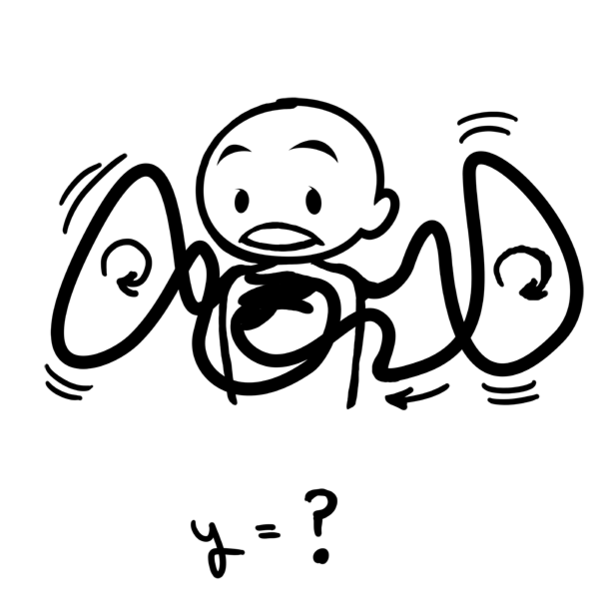
\includegraphics[scale = 0.15]{act_f.png}
\end{transitionframe}

\begin{frame}{Sigmoid activation}
\begin{center}
	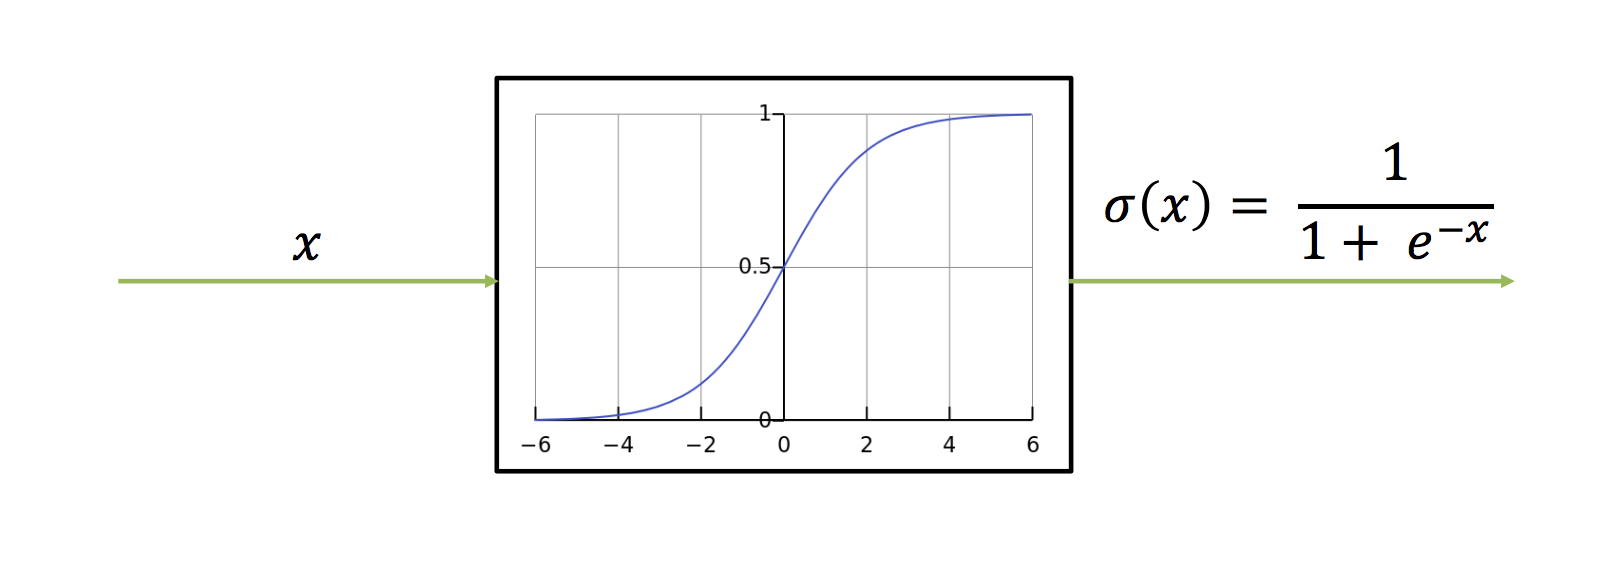
\includegraphics[width=.9\linewidth]{sigmoid_activation_1.png}
\end{center}
\end{frame}

\begin{frame}{Sigmoid activation}
\begin{center}
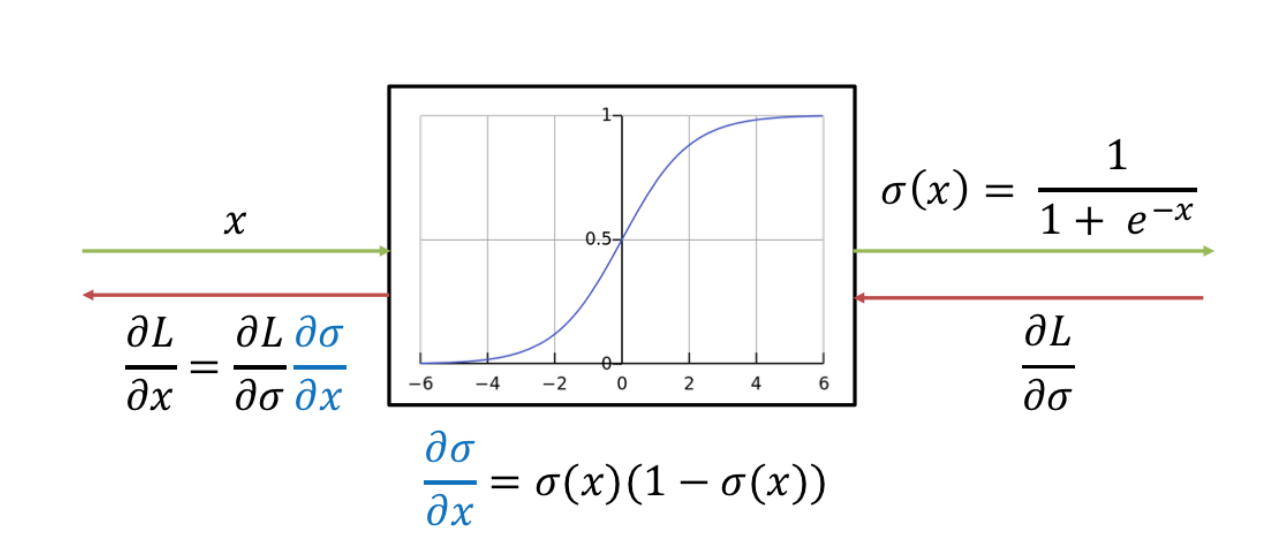
\includegraphics[width=.8\linewidth]{sigmoid_activation_2.png}
\end{center}
\end{frame}


\begin{frame}{Паралич сети}
	\begin{wideitemize}
		\item  В случае сигмоиды $\sigma'(x) = \sigma(x) \cdot (1 - \sigma(x))$ 
		
		\item Сигмоида принимает значения на отрезке $[0; 1]$, значит максимальное значение её производной это $^1/_4$
		
		\item Если сеть очень глубокая, происходит \alert{затухание градиента} 
		
		\item Градиент затухает экспоненциально $\Rightarrow$ сходимость замедляется, более ранние веса обновляются дольше, более глубокие веса быстрее  $\Rightarrow$ значение градиента становится ещё меньше $\Rightarrow$ наступает \alert{паралич сети} 
		
		\item В сетях с небольшим числом слоёв этот эффект незаметен
	\end{wideitemize} 
\end{frame}


\begin{frame}{Затухание градиента (vanishing gradient problem)}

\begin{columns}
	\begin{column}{0.4\textwidth}
		\begin{wideitemize}
			\item  Изменение параметров в ходе обучения происходит на величину, которая никак не влияет на изменение выхода из сетки
			
			\item Проблема связана с очень маленькими градиентами при обновлении весов:
			
			$$
			w_t = w_{t-1} - \gamma \cdot \nabla L(w_{t-1})
			$$
			
		\end{wideitemize}
	\end{column}
	\hfill
	\begin{column}{0.6\textwidth}
		
		\begin{center}
			\only<1>{ 
			$$
			f(t) = \frac{1}{1 + e^{-t}}
			$$
			
			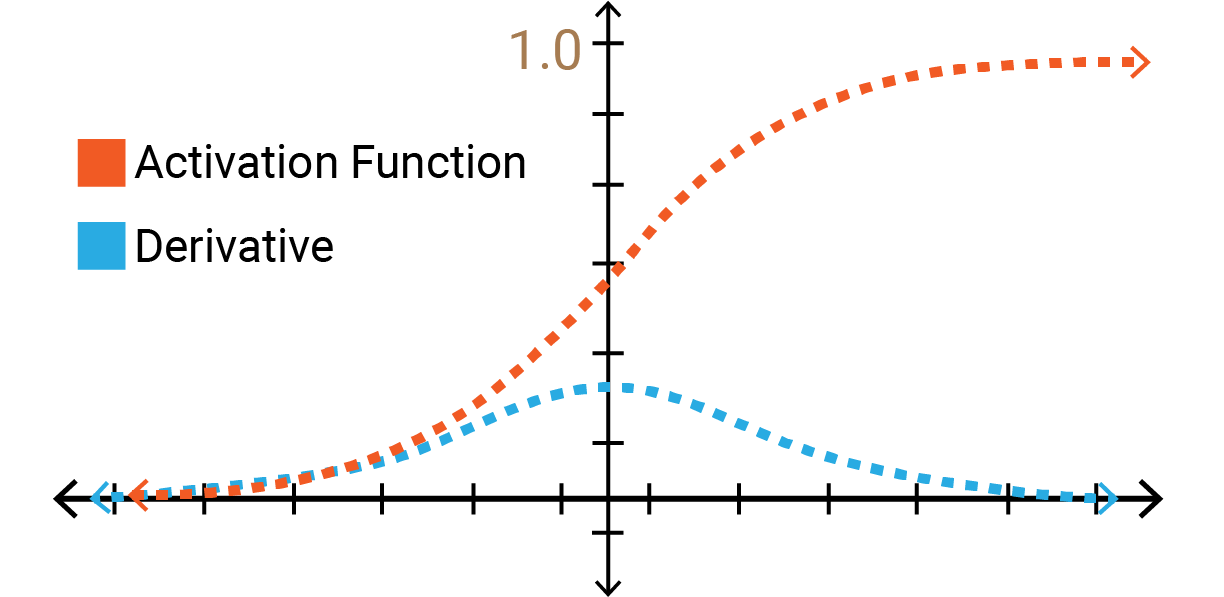
\includegraphics[width=0.98\textwidth]{sigm_der.png} 
			}
		
		% Сделать тут нормальную картинку 
		\only<2>{
			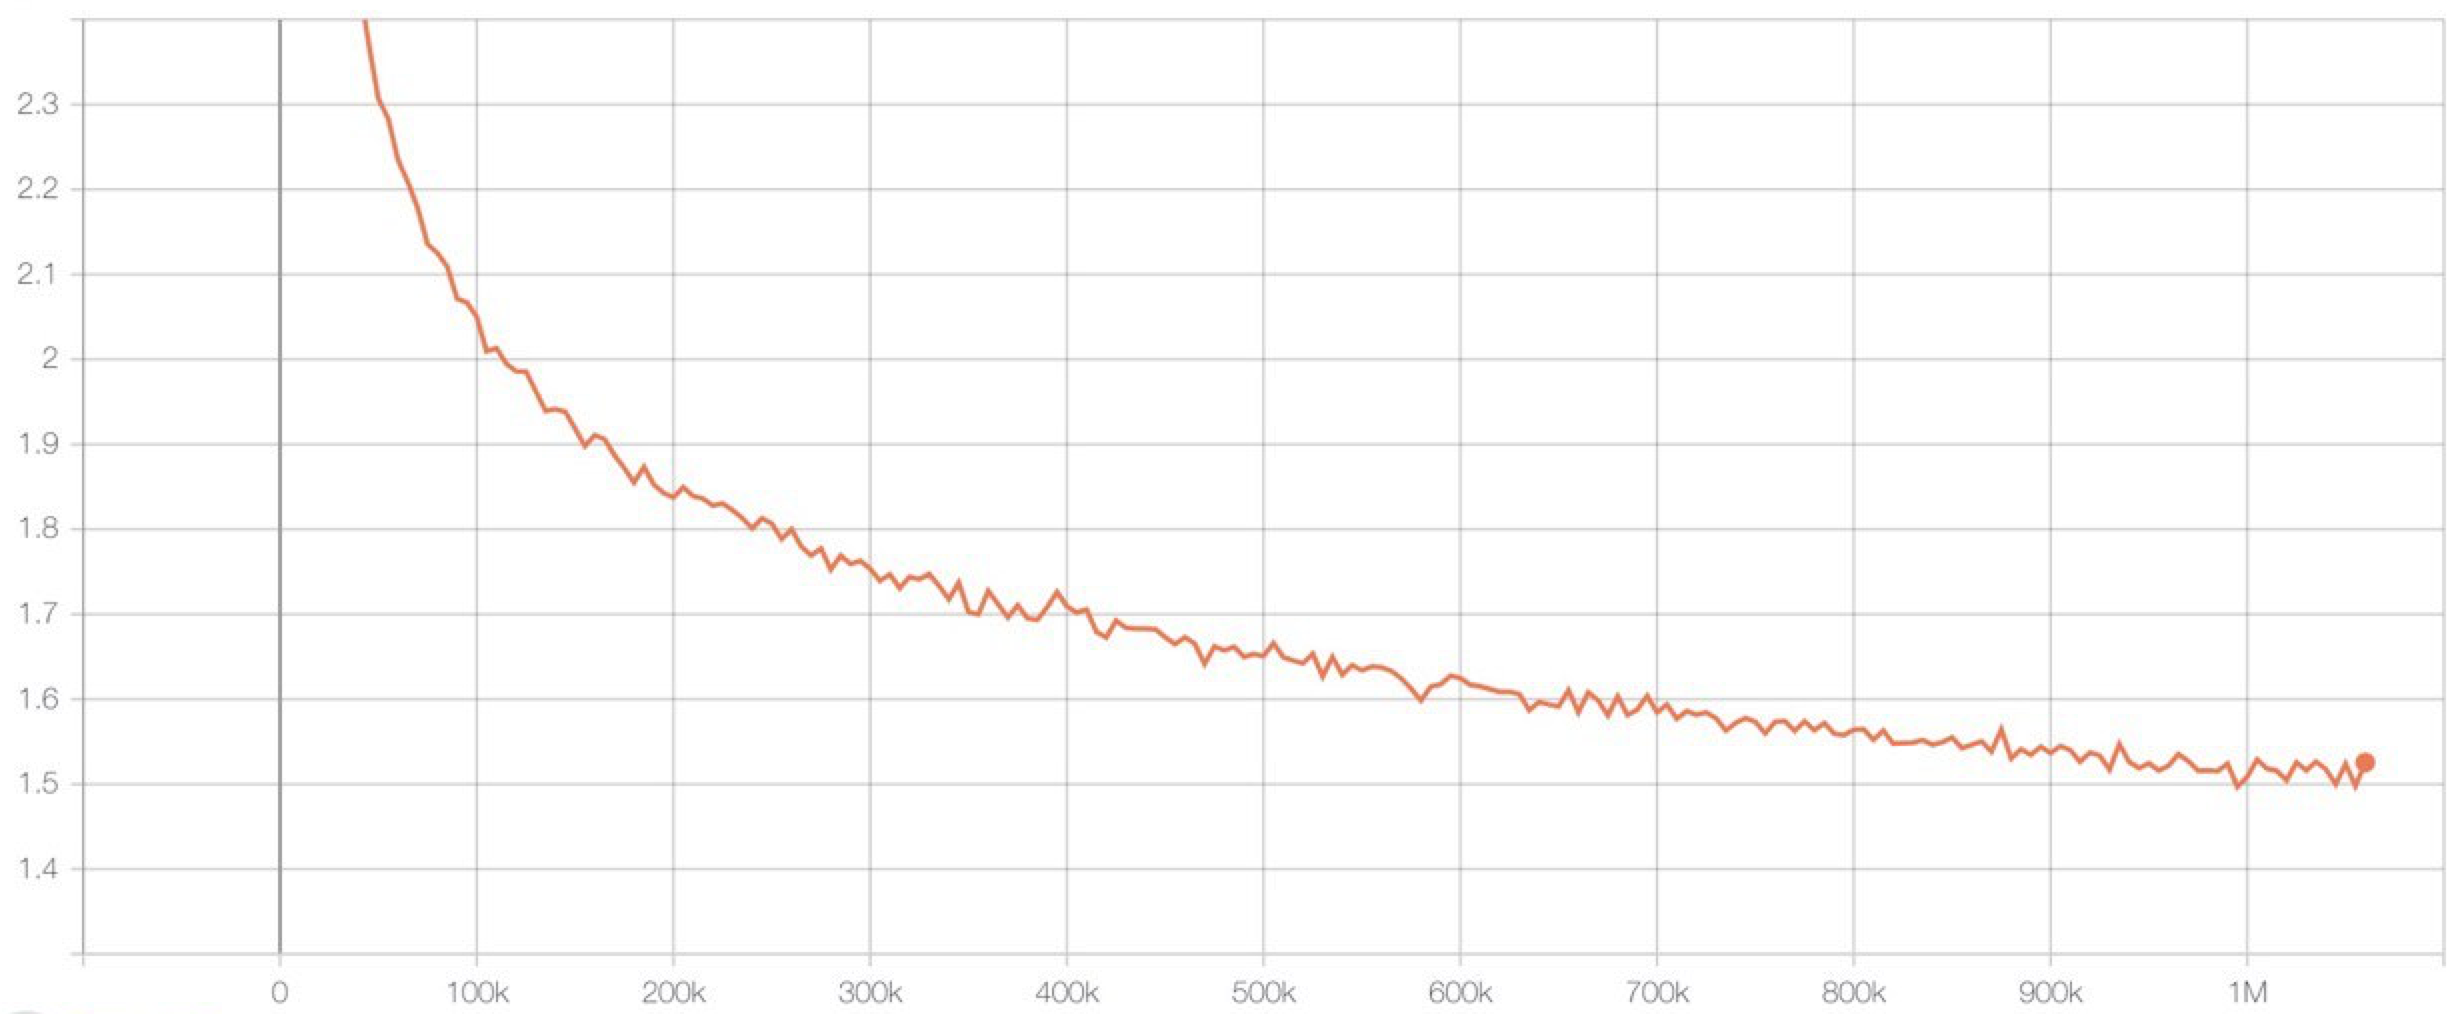
\includegraphics[width=0.98\textwidth]{vanishing_loss.png} 
			
			\mbox{  }
			
			\alert{Толи обучение сошлось, толи веса просто больше не обновляются \ldots}
		}
		\end{center} 
	\end{column}
\end{columns}
\end{frame}



\begin{frame}{Взрыв градиента (exploding gradient problem)}

\begin{columns}
	\begin{column}{0.4\textwidth}
		\begin{wideitemize}
			\item  Изменение параметров в ходе обучения происходит на очень большую величину и обучение деградирует
			
			\item Проблема связана с очень большими градиентами при обновлении весов:
			
			$$
			w_t = w_{t-1} - \gamma \cdot \nabla L(w_{t-1})
			$$
			
		\end{wideitemize}
	\end{column}
	\hfill
	\begin{column}{0.6\textwidth}
		
		\begin{center}
				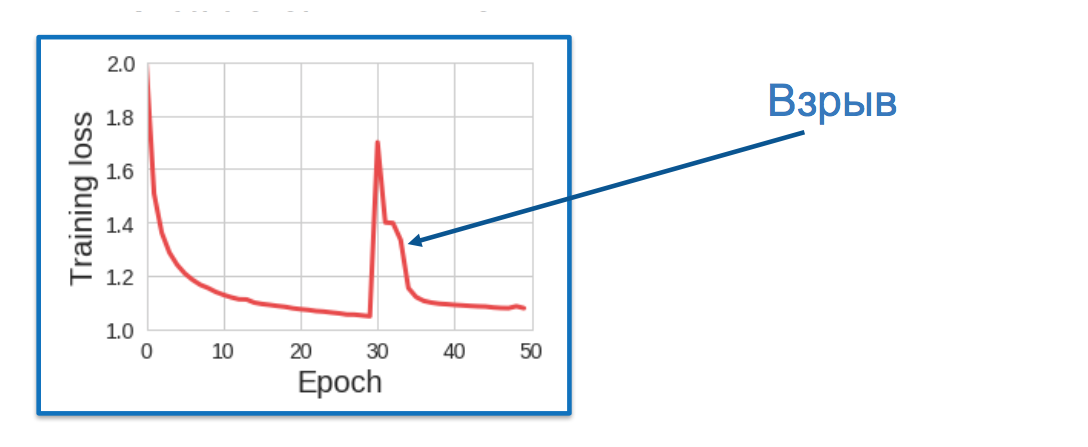
\includegraphics[width=0.98\textwidth]{exp_grad.png} 
		\end{center} 
	\end{column}
\end{columns}
\end{frame}




\begin{frame}{Центрирование}
\begin{wideitemize}
	\item  Сигмоида не центрирована относительно нуля 
	
	\item  Выход слоя мы обычно находим как $o_i = \sigma(h_i)$, он всегда положительный, значит градиент по весам, идущим на вход в текущий нейрон тоже положительные $\Rightarrow$ они обновляются в одинаковом направлении 
	
	\item Сходимость идёт медленнее
\end{wideitemize} 
\end{frame}



\begin{frame}{Sigmoid activation}
\begin{center}
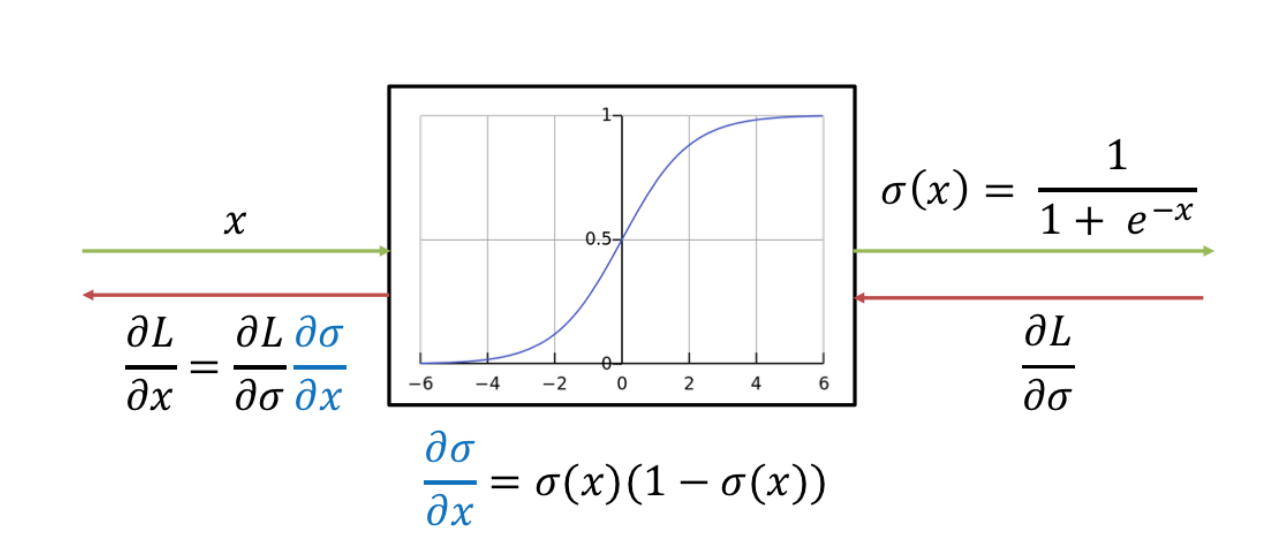
\includegraphics[width=.65\linewidth]{sigmoid_activation_2.png}
\end{center}

\begin{itemize}
{\color{red} 
\item Cпособствует затуханию градиента

\item Не центрирована относительно нуля

\item Вычислять $e^x$ дорого
}
\end{itemize}
\end{frame}


\begin{frame}{Tanh activation}
\begin{center}
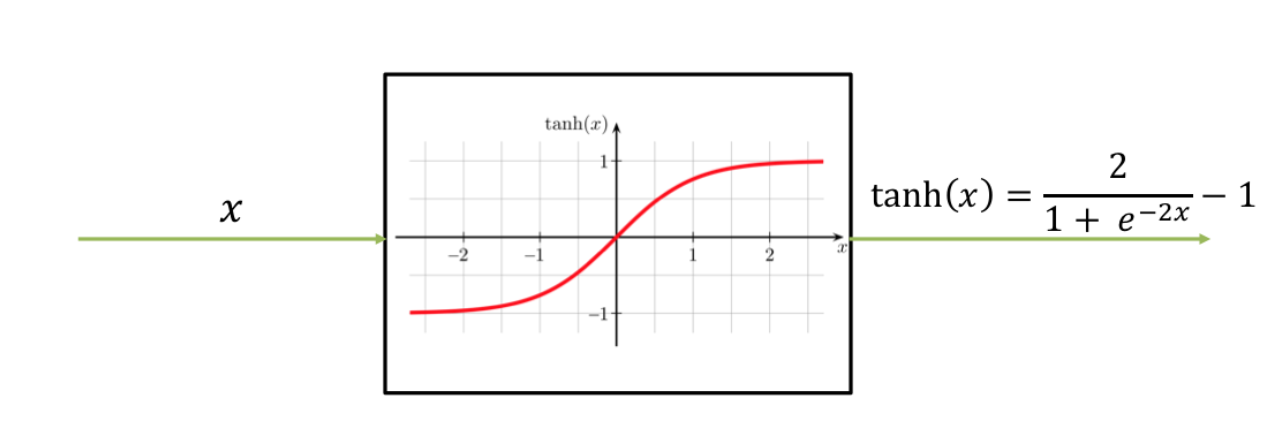
\includegraphics[width=.7\linewidth]{tanh_activation.png}
\end{center}

\begin{itemize}
\item  {\color{green}  Центрирован относительно нуля }

\item  {\color{red}  Всё ещё похож на сигмоиду }

\item $f'(x) = 1 - f(x)^2$  $\Rightarrow$ затухание градиента
\end{itemize}
\end{frame}



\begin{frame}{Rectifier Linear Unit (ReLU) activation}
\begin{center}
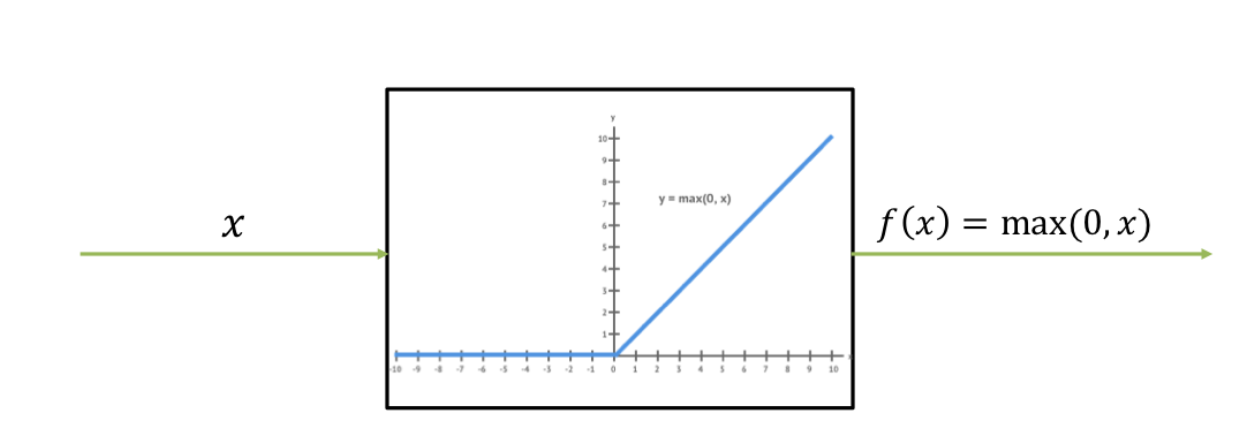
\includegraphics[width=.8\linewidth]{relu_activation.png}
\end{center}

\begin{itemize}
{ \color{green} 
\item  Быстро вычисляется 

\item  Градиент не затухает

\item  Сходимость сеток ускоряется 
} 
\end{itemize}
\end{frame}


\begin{frame}{ReLU activation}
\begin{center}
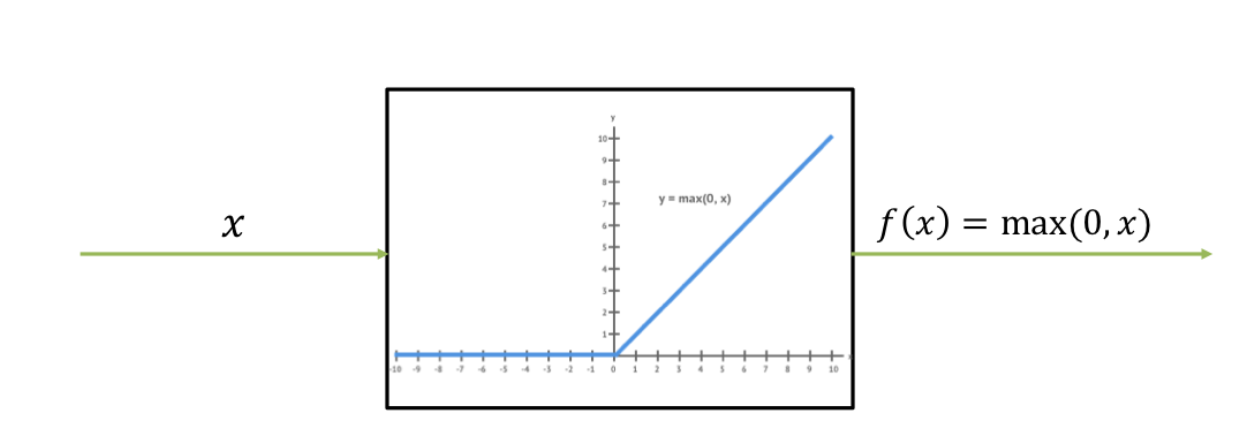
\includegraphics[width=.8\linewidth]{relu_activation.png}
\end{center}

\begin{itemize}
{ \color{red} 
\item  Сетка может умереть, если активация занулится на всех нейронах

\item  Не центрирован относительно нуля
} 
\end{itemize}
\end{frame}


\begin{frame}{Зануление ReLU}
\begin{center}
	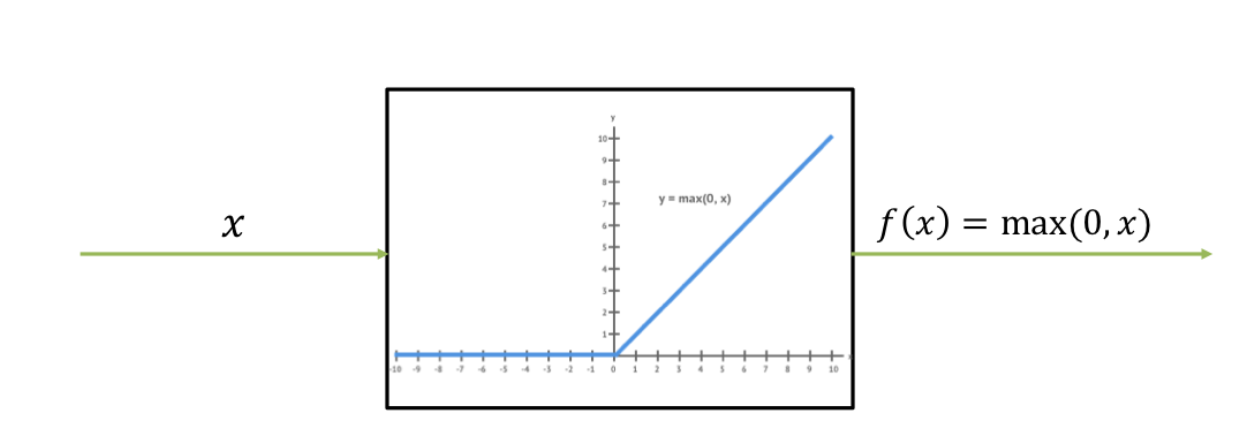
\includegraphics[width=.7\linewidth]{relu_activation.png}
\end{center}

\begin{wideitemize}
	\item   $f(x) = \max(0, w_0 + w_1 \cdot h_1 + \ldots + w_k \cdot h_k)$
	
	\item  Если $w_0$ инициализировано большим отрицательным числом, нейрон сразу умирает $\Rightarrow$ надо аккуратно инициализировать веса
\end{wideitemize}
\end{frame}


\begin{frame}{Leaky ReLU activation}
\begin{center}
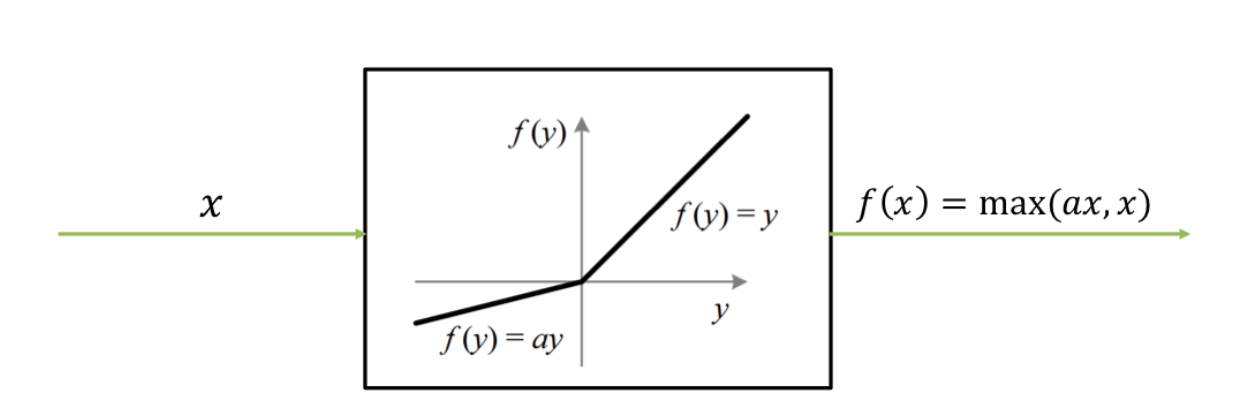
\includegraphics[width=.7\linewidth]{leaky_relu_activation.png}
\end{center}

\begin{itemize}
{ \color{green} 
\item Как ReLU, но не умирает, всё ещё легко считается
\item Производная может быть любого знака
\item Важно, чтобы $a \ne 1$, иначе линейность
} 
\end{itemize}
\end{frame}


\begin{frame}{Leaky ReLU activation}
\begin{columns}
	\begin{column}{0.4\textwidth}
		\begin{wideitemize}
			\item  При использовании ReLU градиенты не взрываются и не затухают, они при проходе через этот слой всегда равны константе
			
			$$
			w_t = w_{t-1} - \gamma \cdot \nabla L(w_{t-1})
			$$
			
		\end{wideitemize}
	\end{column}
	\hfill
	\begin{column}{0.6\textwidth}
		
		\begin{center}
			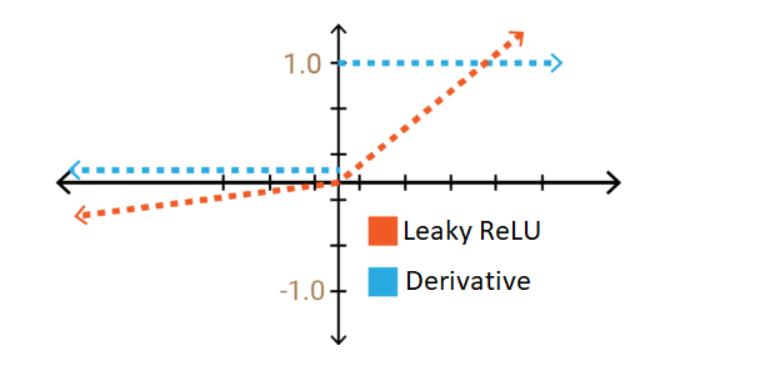
\includegraphics[width=0.98\textwidth]{leaky_relu_der.png} 
		\end{center} 
	\end{column}
\end{columns}
\end{frame}


% слайд очень хуёво выглядит внешне
\begin{frame}{Exponential linear unit (ELU) activation}
\begin{columns}
	\begin{column}{0.6\textwidth}
		\begin{center}	
		\begin{wideitemize}
			\item Функция "примерно центрирована" относительно нуля
			\item Это позволяет избегать "смещения" в положительном направлении и ускоряет обучение 
		\end{wideitemize}
			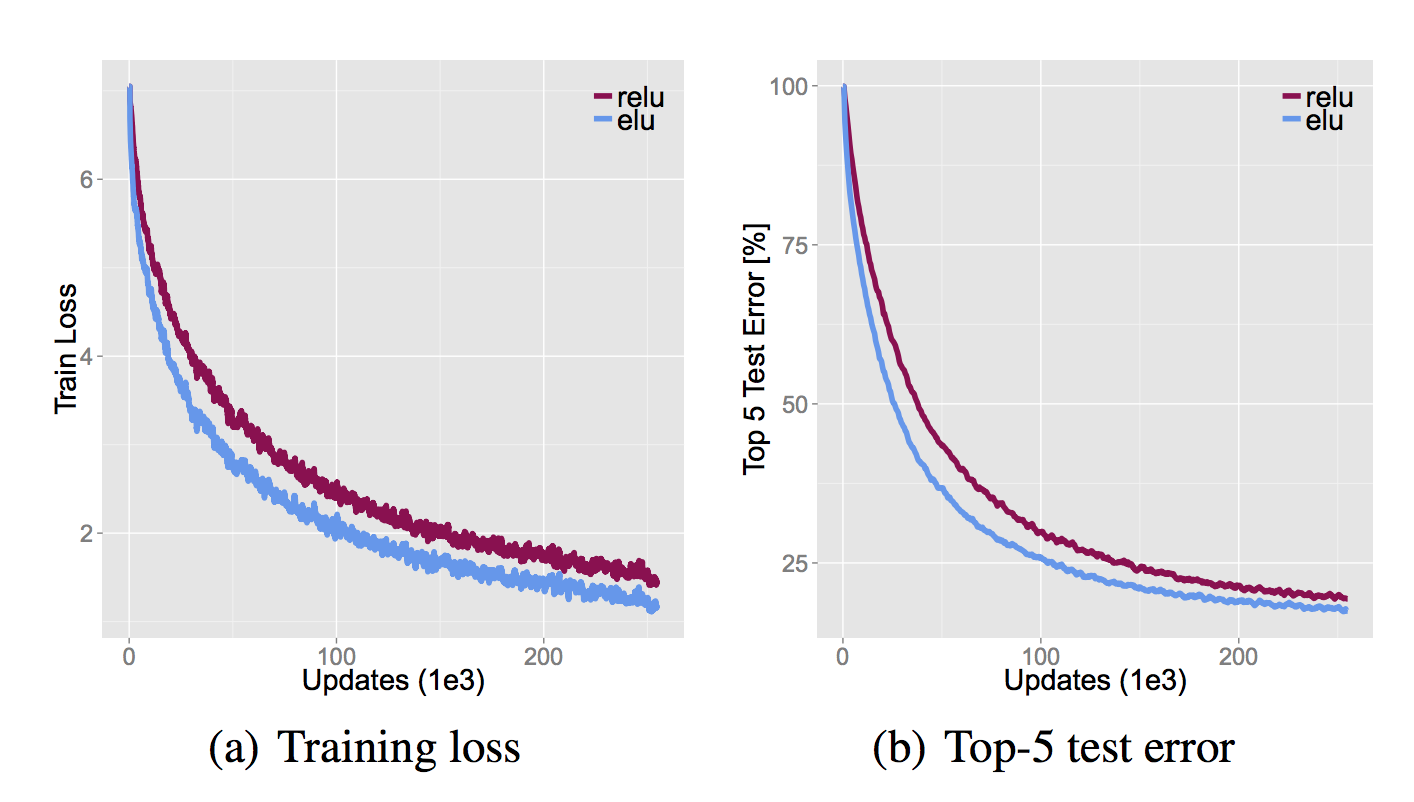
\includegraphics[width=.7\linewidth]{elu_loss.png}
	\end{center}
	\end{column}
	\hfill
	\begin{column}{0.4\textwidth}
			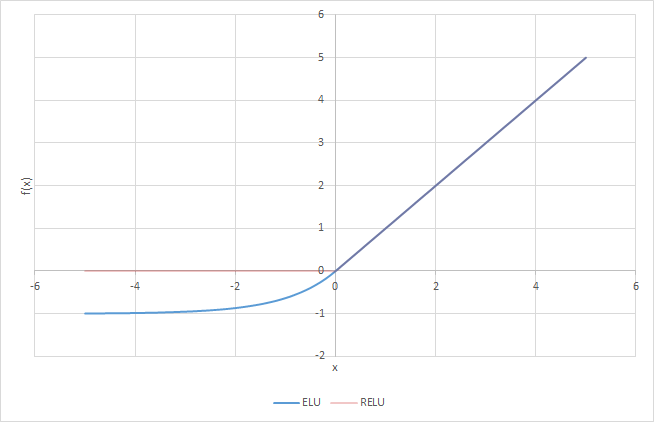
\includegraphics[width=.8\linewidth]{elu.png}
			
			$$
			f(x) = \begin{cases} x,  x \ge 0 \\ \alpha \cdot (e^x - 1),  x < 0 \end{cases}
			$$
	\end{column}
\end{columns}

\vfill %
\footnotesize
{\color{blue} \url{https://arxiv.org/pdf/1511.07289.pdf}}
\end{frame}





%\begin{frame}{Что же выбрать}
%\begin{wideitemize}
%	\item Обычно начинают с $ReLU$, если сетка умирает, берут $Leaky ReLU$
%	\item $ReLU$ — стандартный выбор для свёрточных сетей 
%	\item В рекурентных сетках чаще всего предпочитается $tanh$ 
%	\item На самом деле это не очень важно, нужно держать в голове свойства функций, о которых выше шла речь и понимать, что от перебора функций обычно выигрыш в качестве довольно низкий 
%	\item Но есть и исключения ...
%\end{wideitemize}
%
%\vfill %
%\footnotesize
%Краткий обзор функций активаций: {\color{blue}  \url{https://arxiv.org/pdf/1804.02763.pdf}}
%\end{frame}







%\begin{frame}{Swish activation}
%\begin{wiseitemize}
%	\item В 2017 году Google Brain с помощью хитрого автоматического поиска на основе RNN нашла функцию активации Swish, которая оказалась заметно лучше ReLU
%	
%	$$
%	f(x) = x \cdot \sigma(\beta \ cdot x)
%	$$
%	
%	\item Проапгрейдили сигмоиду ко ко ко 
%	
%\end{wiseitemize}
%
%\begin{center}
%	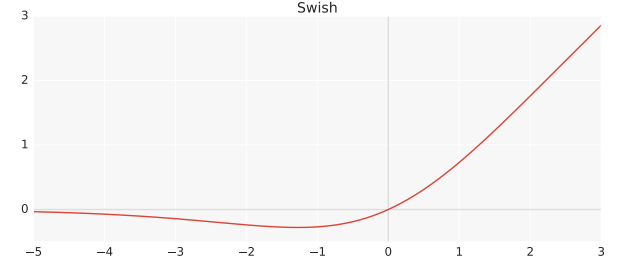
\includegraphics[width=.4\linewidth]{swish.png}
%\end{center}
%
%
%\vfill %
%\footnotesize
%{\color{blue} \url{https://arxiv.org/abs/1710.05941} \newline \url{https://krutikabapat.github.io/Swish-Vs-Mish-Latest-Activation-Functions/} }
%\end{frame}


%Activate or Not: Learning Customized Activation
%Ningning Ma, Xiangyu Zhang, Jian Sun
%Статья: https://arxiv.org/abs/2009.04759 
%
%Давно мы не писали про какие-нибудь хитрые функции активации, а вернее, кажется, вообще не писали ни разу. А тут и повод есть.
%
%В 2017 году команда из Google Brain с помощью хитрого автоматического поиска, построенного на RNN-ках, нашла функцию активации Swish [f(x) = x · sigmoid(βx)], которая оказалась заметно лучше ReLU (https://arxiv.org/abs/1710.05941).
%
%Поскольку никакой человек эту функцию не дизайнил, спросить RNN-ку, что она имела в виду, не получается. Работает и работает, а GPT-3 для объяснения результатов нейро-поиска ещё никто не прикручивал вроде.
%
%Функция стала популярна, её часто можно встретить у тех, кто старается выжать последние проценты качества из имеющихся моделей. Затем подоспело ещё какое-то число свежих функций, например, Mish, которая вроде как ещё лучше (https://krutikabapat.github.io/Swish-Vs-Mish-Latest-Activation-Functions/).
%
%И вот на днях появилось логическое продолжение под названием ACON.
%
%В чём дело? Разберёмся!
%
%Подход в общем классический. Давайте поймём как имеющиеся функции можно обобщить, а потом из этого обобщения предложим что-нибудь интересное. Заодно и интуицию обретём.
%
%Логические шаги тут следующие:
%
%1. Функцию max можно аппроксимировать гладким и дифференцируемым вариантом, который мы будем называть smooth maximum с параметром β, который когда стремится к бесконечности, даёт в пределе максимум, а когда стремится к нулю — арифметическое среднее.
%
%S_β(x_1, ..., x_n) = sum(x_i*exp(β*x_i))/sum(exp(β*x_i))
%
%2. ReLU это, как известно, max(x,0), а значит можно аппроксимировать этим нашим гладким максимумом о двух входах: 
%
%S_β(η_a(x), η_b(x))
%и η_a(x) = x, η_b(x) = 0,
%
%3. Swish тоже можно представить через эту функцию S_β(x, 0) = x * σ(β*x) и её мы называем ACON-A. А заодно Swish — это гладкая аппроксимация ReLU.
%
%4. Если рассмотреть развития ReLU типа PReLU, Leaky ReLU и т.п., то можно прийти к функции ACON-B c n η_a(x) = x, η_b(x) = px.
%
%5. Можно пойти ещё дальше и сделать ACON-C с η_a(x) = p_1*x, η_b(x) = p_2*x(p_1 != p_2). ACON-C в такой формулировке позволяет иметь обучаемые верхние и нижние границы для градиента (у Swish они фиксированы). Они определяются параметрами p_1 и p_2.
%
%6. Ну и наконец параметр β тоже можно обучать и это даёт функцию Meta-ACON. Этот параметр называется switching factor и регулирует поведение нейрона: линейный (неактивный нейрон) или нелинейный режим работы (активный нейрон). Отсюда и название ActivateOrNot (ACON).
%
%И вот эта последняя история открывает целое пространство для исследования, можно реализовывать разные функции, генерящие эту β по входным данным: можно иметь общий параметр на весь слой, можно на отдельные каналы, а можно и на пиксели.
%
%Что вообще даёт вся эта эквилибристика? На редкость неплохие улучшения, единицы процентных пунктов в терминах top-1 ошибки. Для которых от вас по большому счёту ничего не требуется кроме замены функции активации.
%
%Ну и заодно вроде понятнее стало, что такое Swish и вообще.


\begin{transitionframe}
	\begin{center}
		\Huge  Батч-нормализация
	\end{center}
	\centering 
\includegraphics[scale = 0.25]{batcAlice.png}
\end{transitionframe}


\begin{frame}{Стандартизация}
\begin{center}
	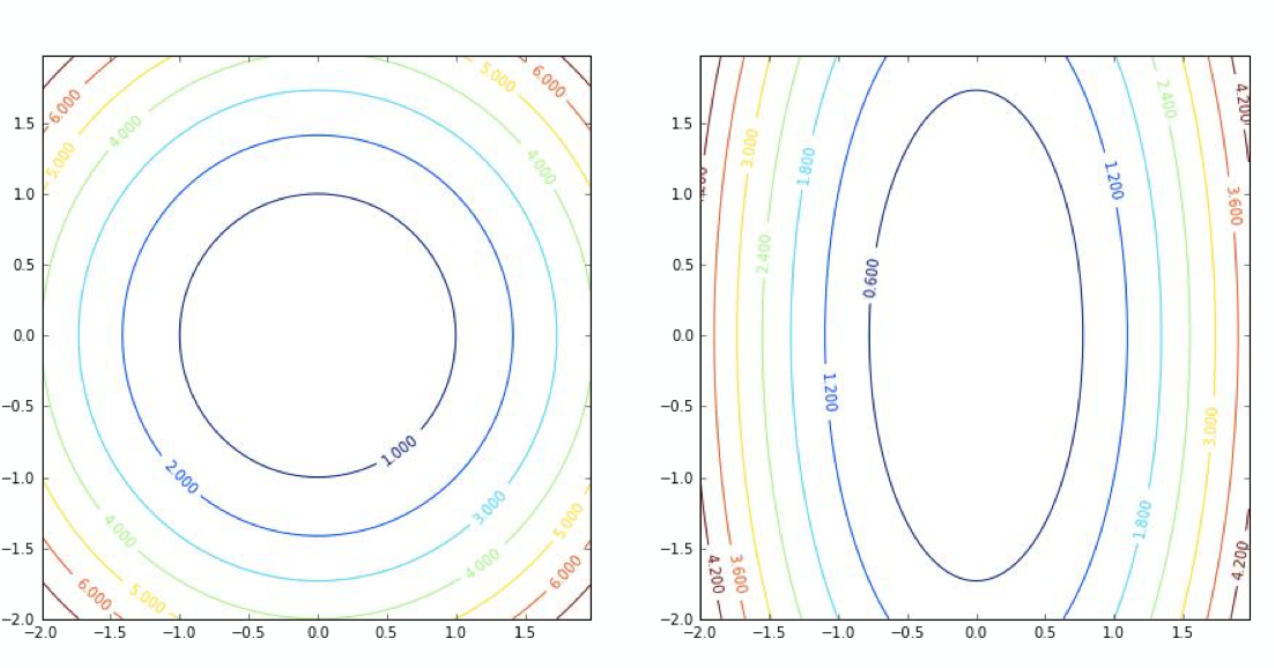
\includegraphics[width=.8\linewidth]{standartization.png}
\end{center}

\begin{center}
	Какая из ситуаций лучше для SGD? 
\end{center}
\end{frame}


\begin{frame}{Стандартизация}
\begin{center}
	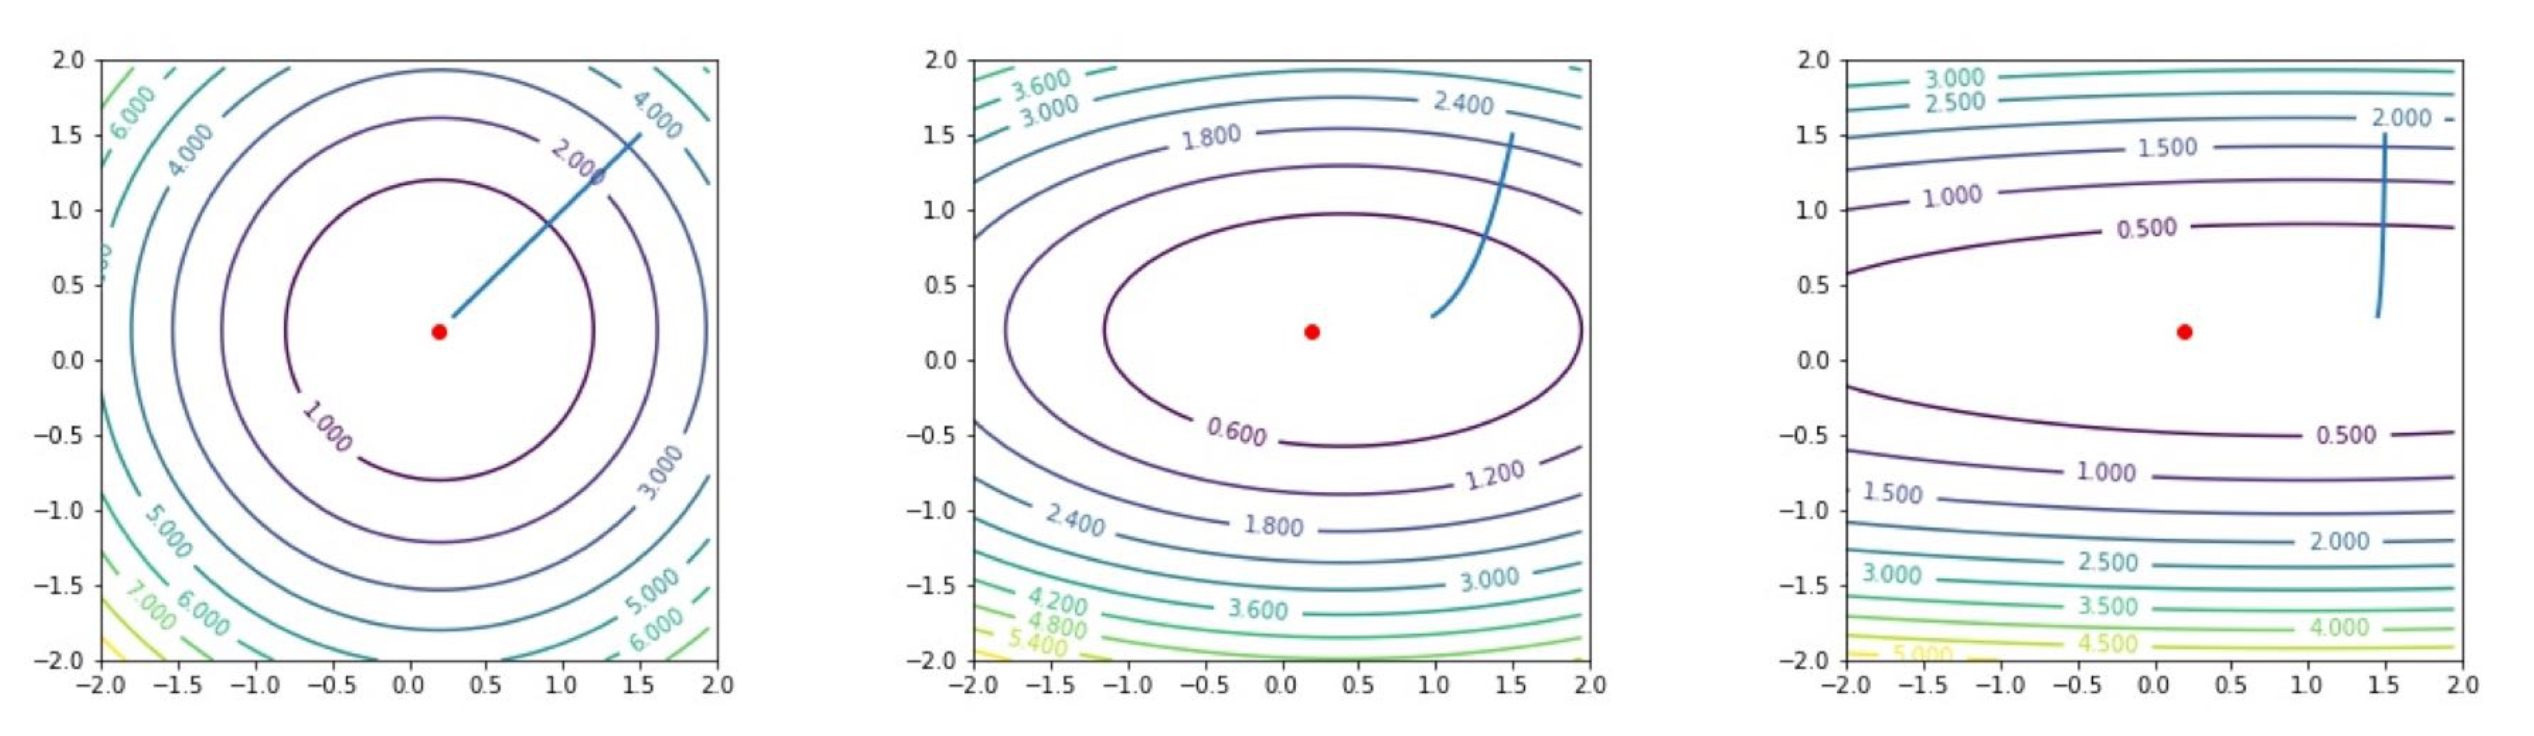
\includegraphics[width=.99\linewidth]{standartization2.png}
\end{center}

\alert{Градиентные методы быстрее сходятся, если градиенты в одном масштабе}

\vfill %
\footnotesize
{\color{blue} \url{https://github.com/hse-aml/intro-to-dl/blob/master/week2/v2/ill-conditioned-demo.ipynb}}
\end{frame}


\begin{frame}{А что внутри нейросетки?}
\begin{center}
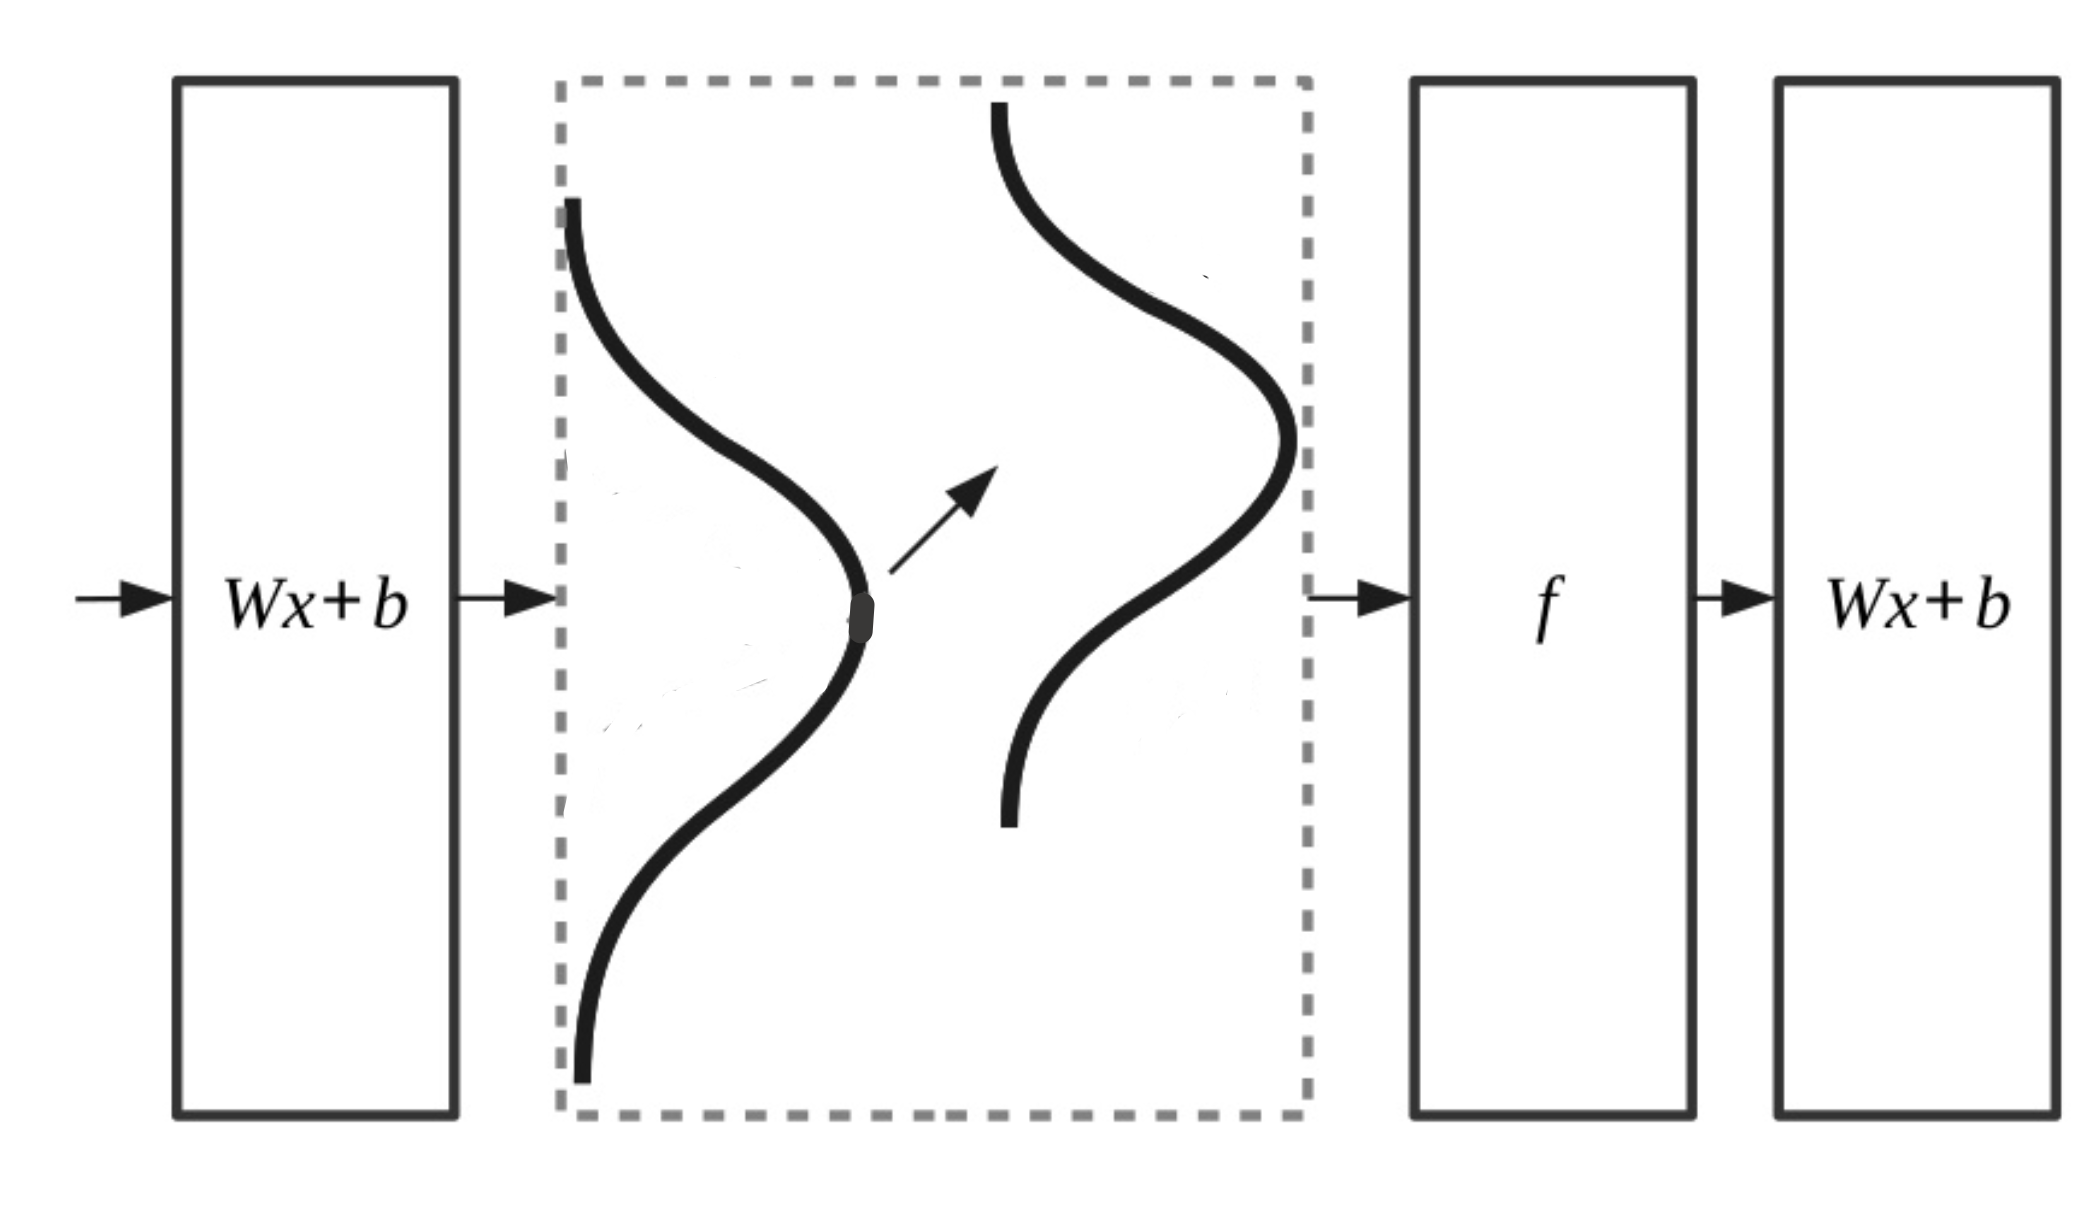
\includegraphics[width=.7\linewidth]{distributions_1.png}
\end{center}
\end{frame}


\begin{frame}{А что внутри нейросетки?}
\begin{center}
	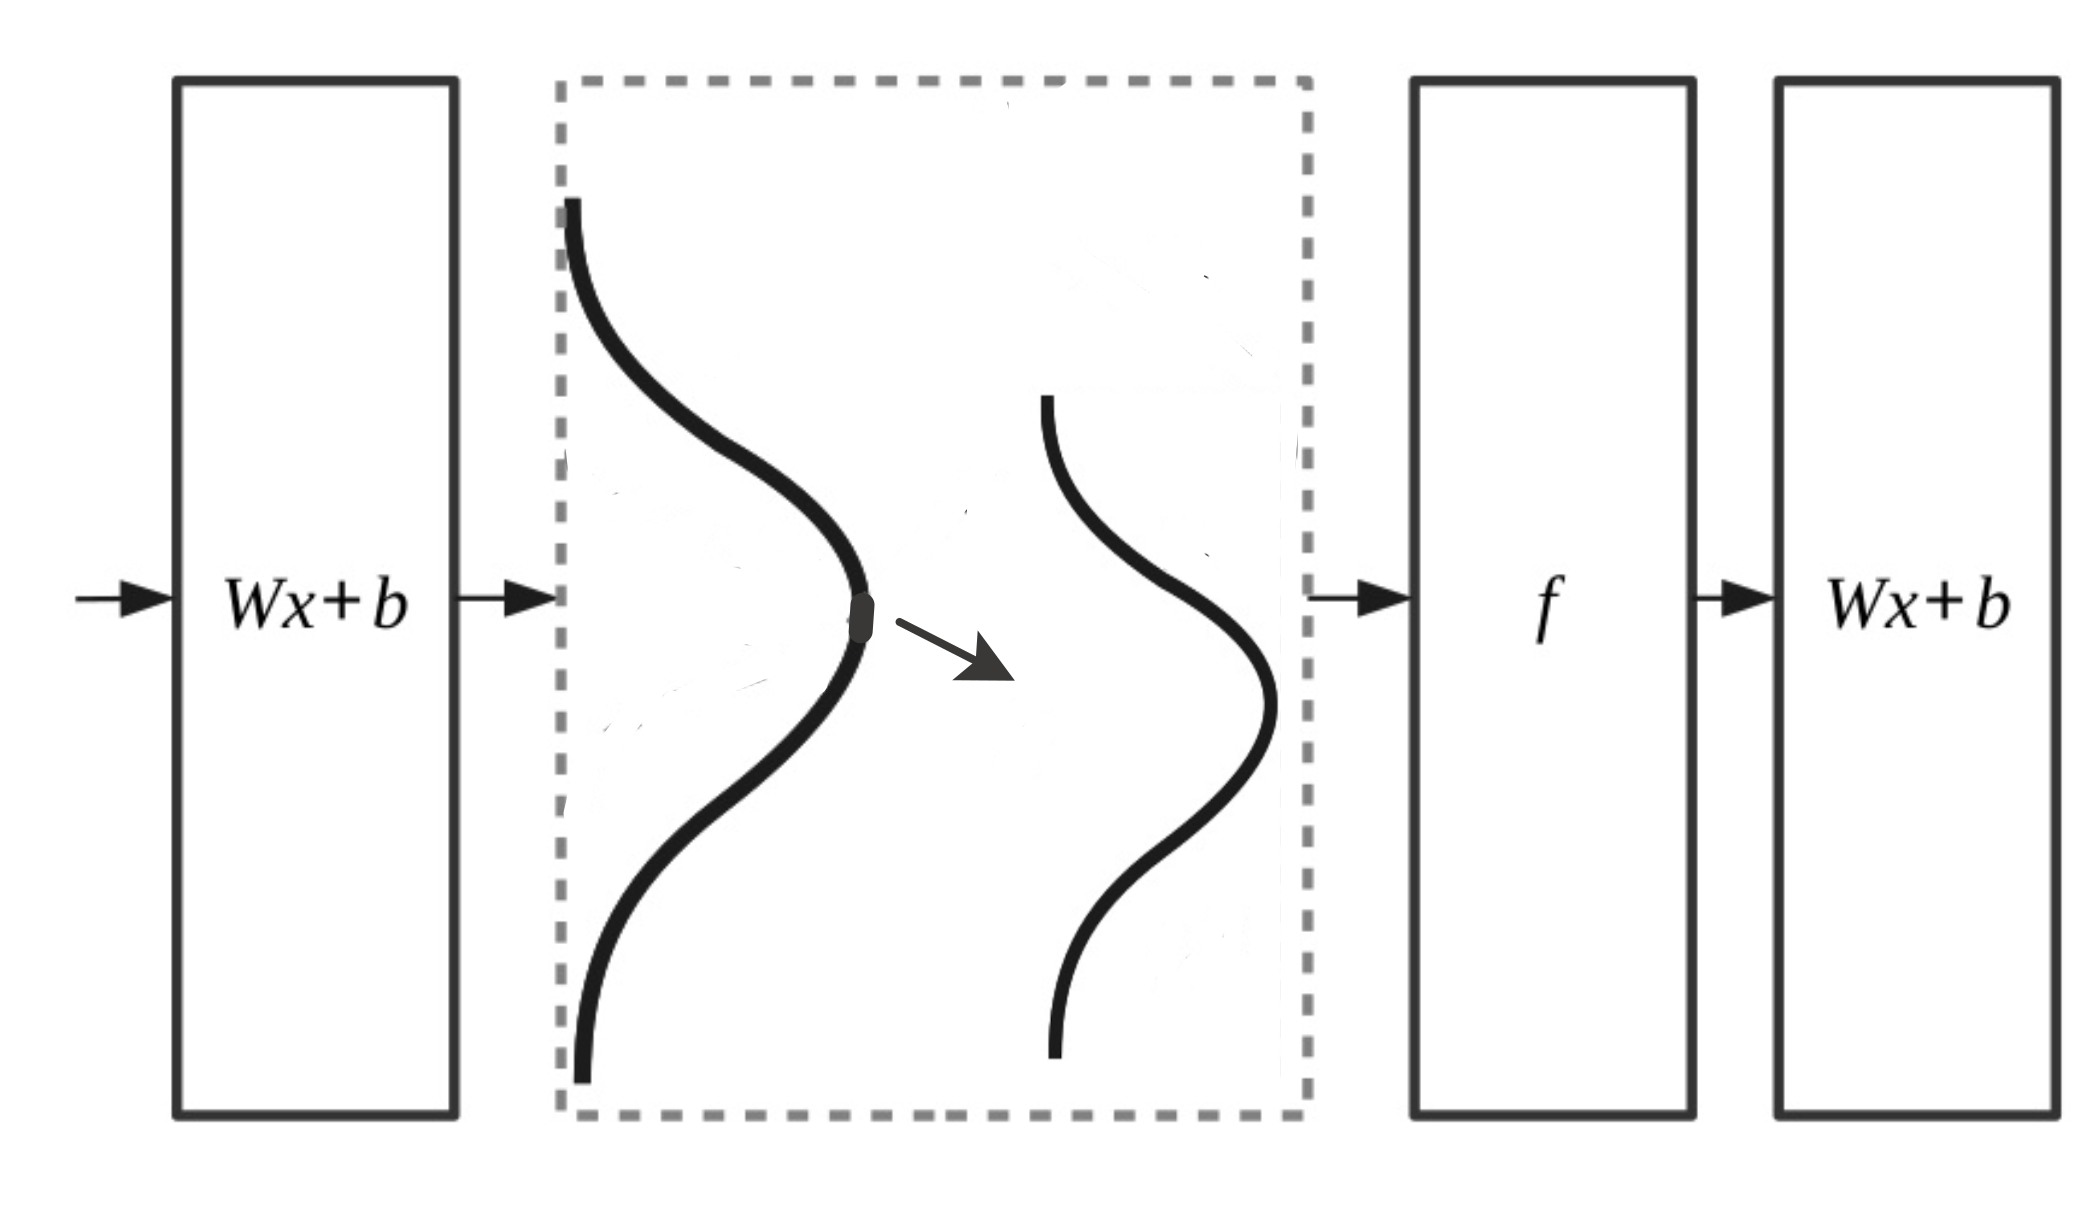
\includegraphics[width=.7\linewidth]{distributions_2.png}
\end{center}
\end{frame}


\begin{frame}{Проблема}
\begin{wideitemize}
	\item Давайте вместо $X$ на входе использовать $\frac{X - \mu_X}{\sigma_X}$
	
	\item  Даже если мы стандартизовали вход $X$, внутри сетки может произойти несчастье и скрытый слой окажется нестандартизован 
	
	\item  Скрытые представления $h = f(XW)$  могут менять своё распределение в процессе обучения, это усложняет его  \pause
	
	\item Давайте на каждом слое вместо $h$ использовать  $\hat h = \frac{h - \mu_h}{\sigma_h}$
	
	\item На выход будем выдавать $\beta \cdot  \hat h + \gamma$, для того, чтобы у нас было больше свободы, параметры $\beta$ и $\gamma$ тоже учим 
\end{wideitemize}
\end{frame}


\begin{frame}{Batch norm (2015)}
\begin{center}
	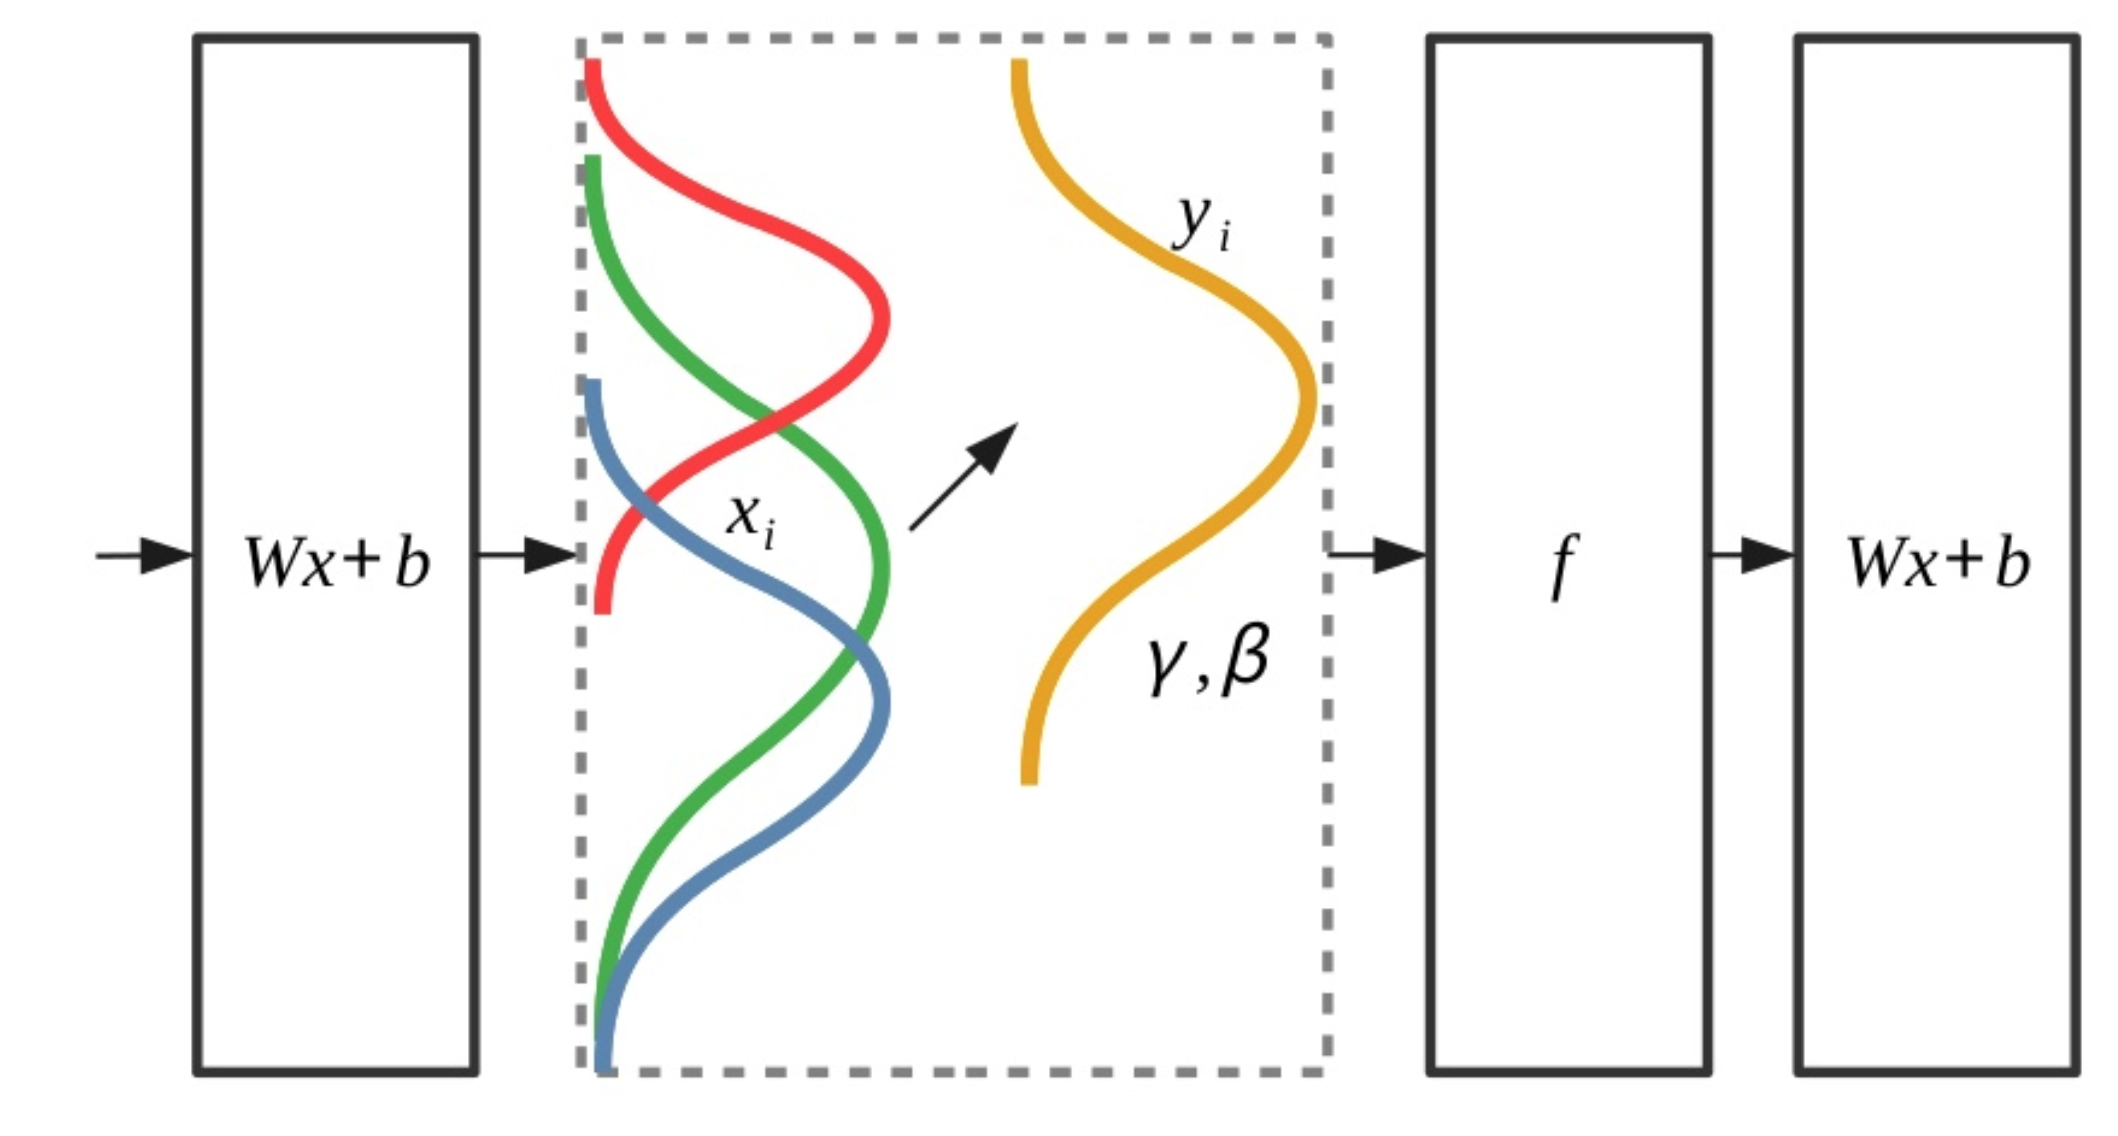
\includegraphics[width=.7\linewidth]{distributions_nice.png}
\end{center}
\end{frame}

\begin{frame}{Forward pass}
\begin{center}
	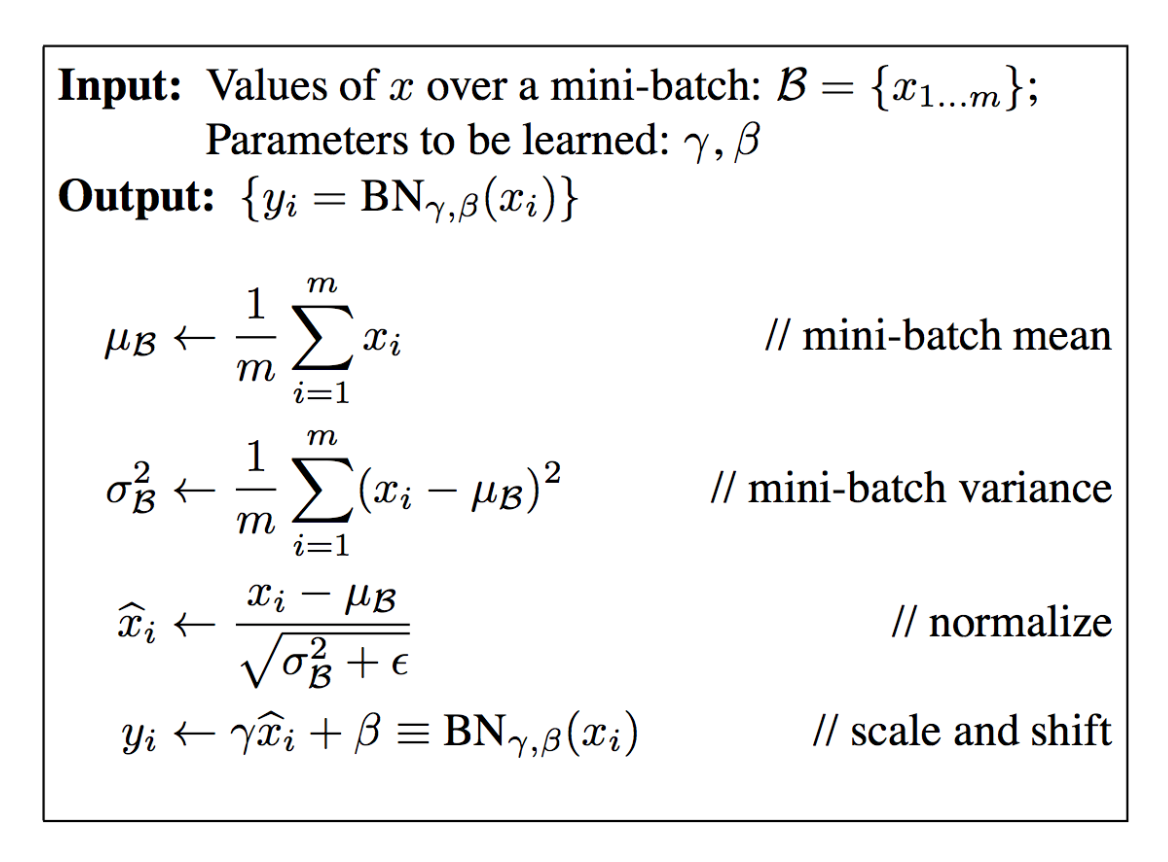
\includegraphics[width=.6\linewidth]{batch_formulas.png}
\end{center}
\vfill %
\footnotesize
{\color{blue} \url{https://arxiv.org/pdf/1502.03167.pdf}}
\end{frame}


\begin{frame}{Backward pass}
\begin{center}
	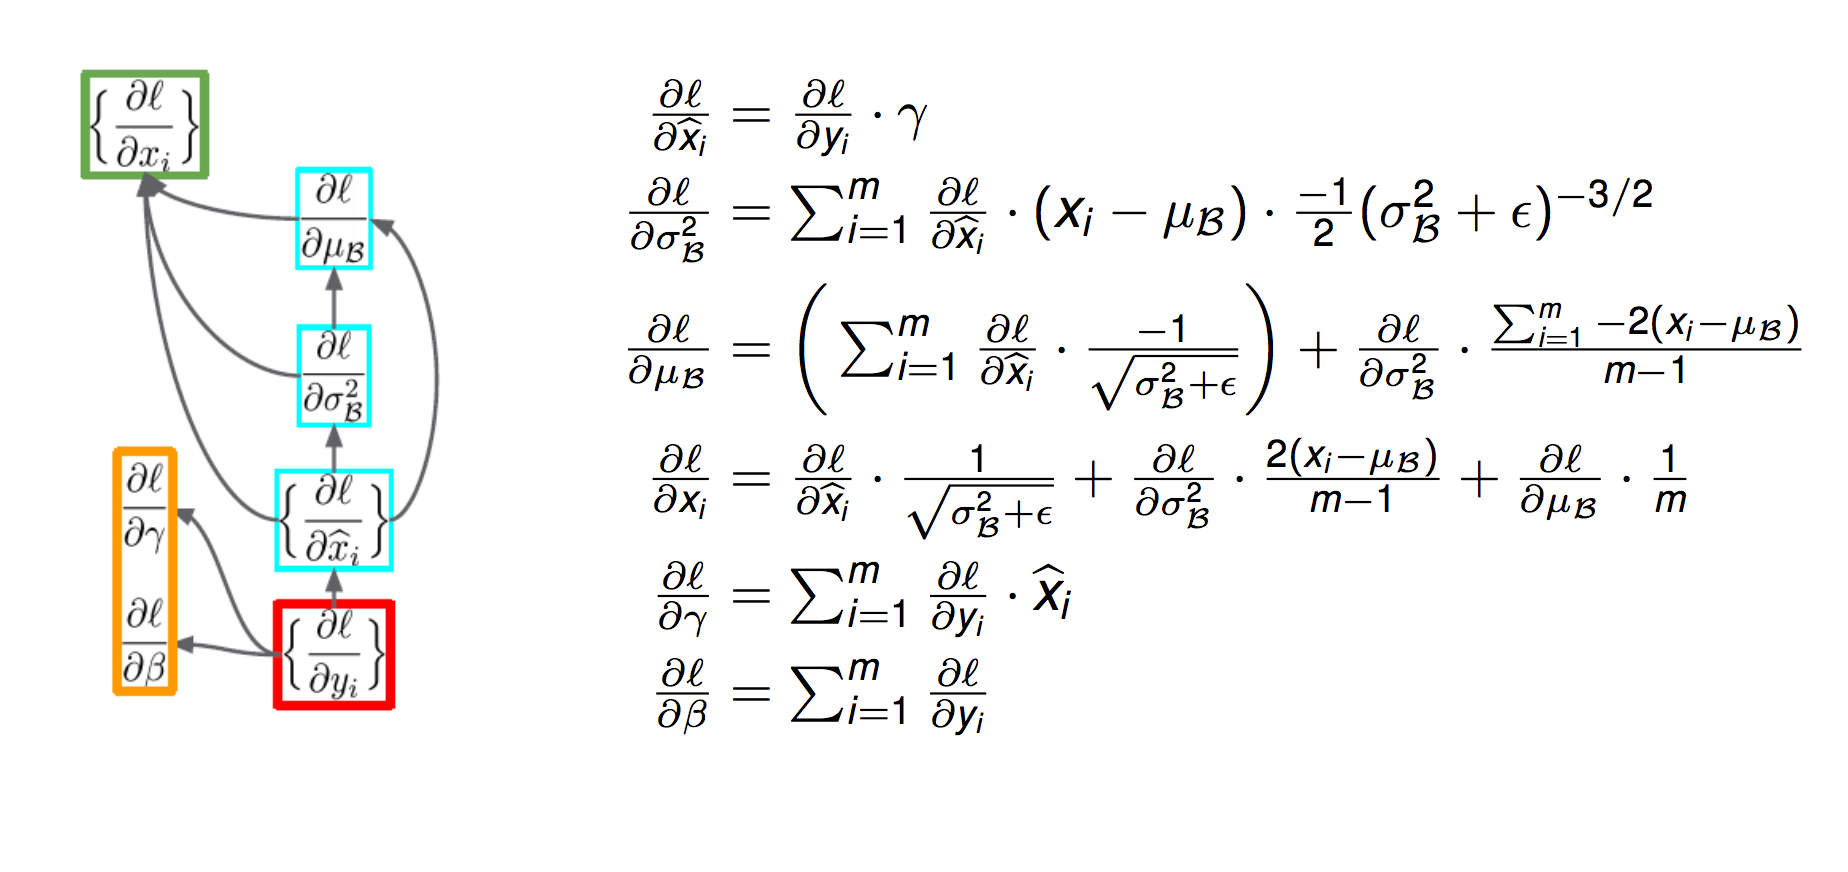
\includegraphics[width=.95\linewidth]{batch_grad.png}
\end{center}
\vfill %
\footnotesize
{\color{blue} \url{https://arxiv.org/pdf/1502.03167.pdf}}
\end{frame}

\begin{frame}{Batch norm (2015)}
\begin{wideitemize}
	\item  Как считать $\mu_h$ и $\sigma_h$? 
	
	\item Оценить по текущему батчу! 
	
	\begin{align*} 
	\mu_h =  \alpha \cdot \bar x_{batch}  + (1 - \alpha) \cdot \mu_h \\ 
	\sigma_h =  \alpha \cdot \hat s_{batch}  + (1 - \alpha) \cdot \sigma_h \\ 
	\end{align*}
	
	\item Коэффициенты $\beta$ и $\gamma$ оцениваются в ходе обратного распространения ошибки, $\mu$ и $\sigma$ не обучаются
	
	\item Обучение довольно сильно ускоряется, сходимость улучшается 
\end{wideitemize}

\vfill %
\footnotesize
{\color{blue} \url{https://arxiv.org/pdf/1502.03167.pdf}}
\end{frame}

\begin{frame}{Эксперимент с MNIST}
\begin{center}
	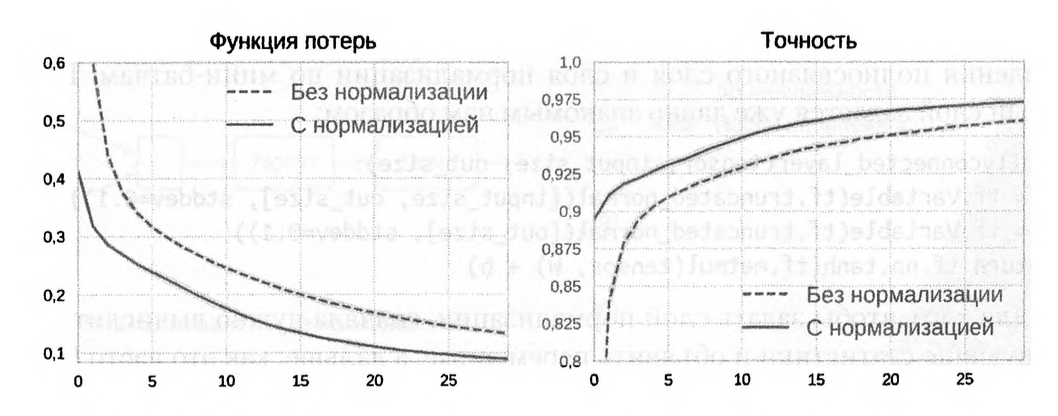
\includegraphics[width=.8\linewidth]{batch_norm.png}
\end{center}
\vfill
{\small  Источник: Николенко, страница 160}
\end{frame}


\begin{frame}{Почему это помогает при обучении}
\begin{center}
	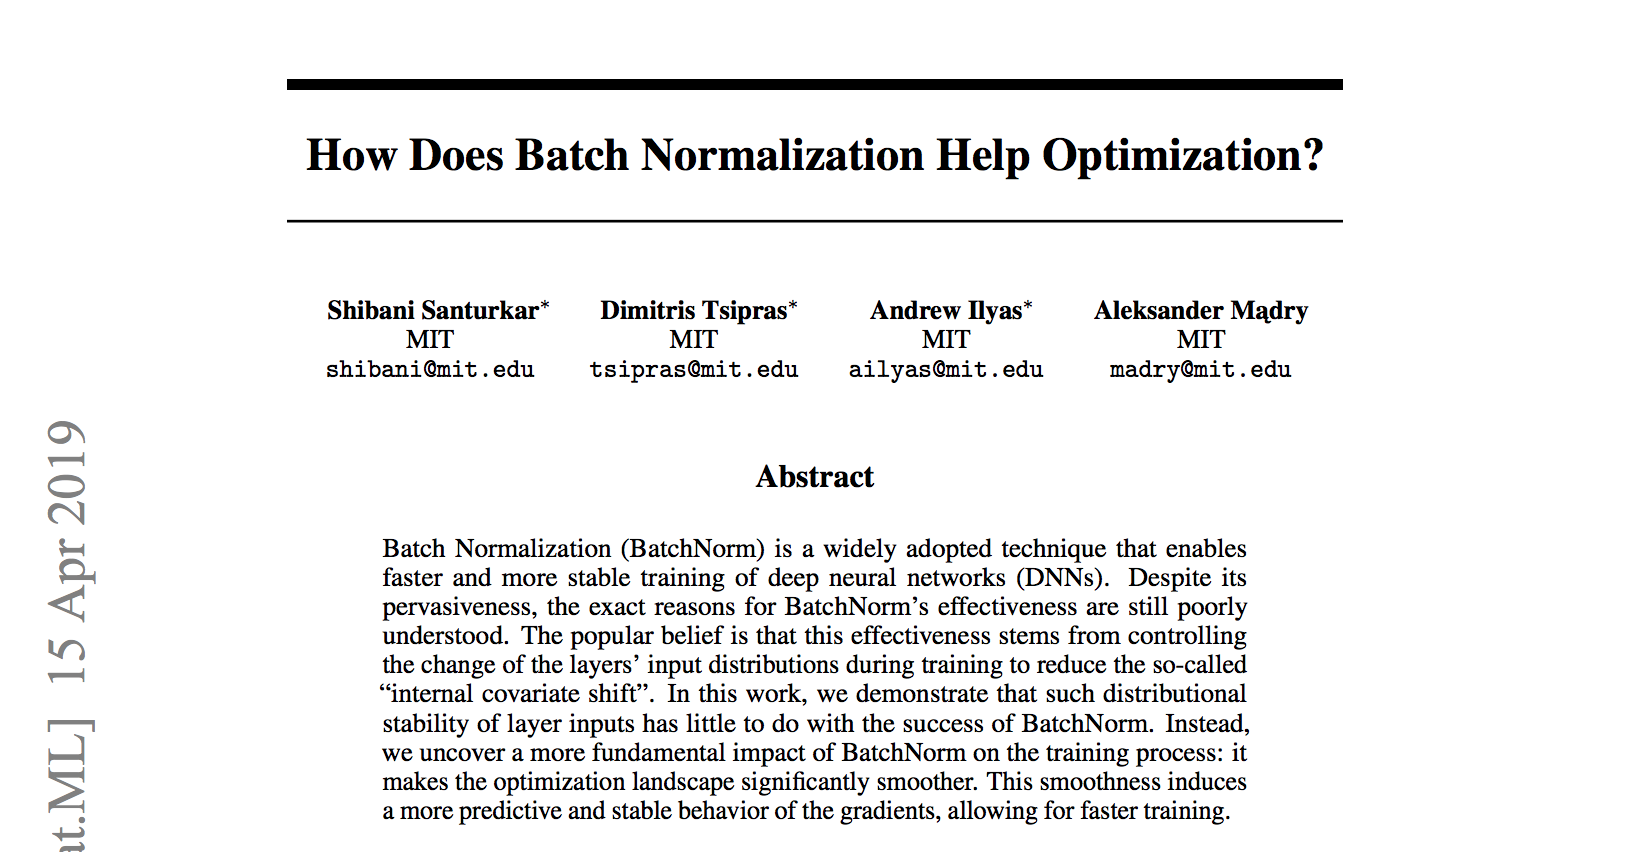
\includegraphics[width=.8\linewidth]{how_bn_help.png}
\end{center}
\vfill
\footnotesize
{\color{blue} \url{https://arxiv.org/abs/1805.11604}}
\end{frame}


\begin{frame}{Почему это помогает при обучении}
\begin{center}
	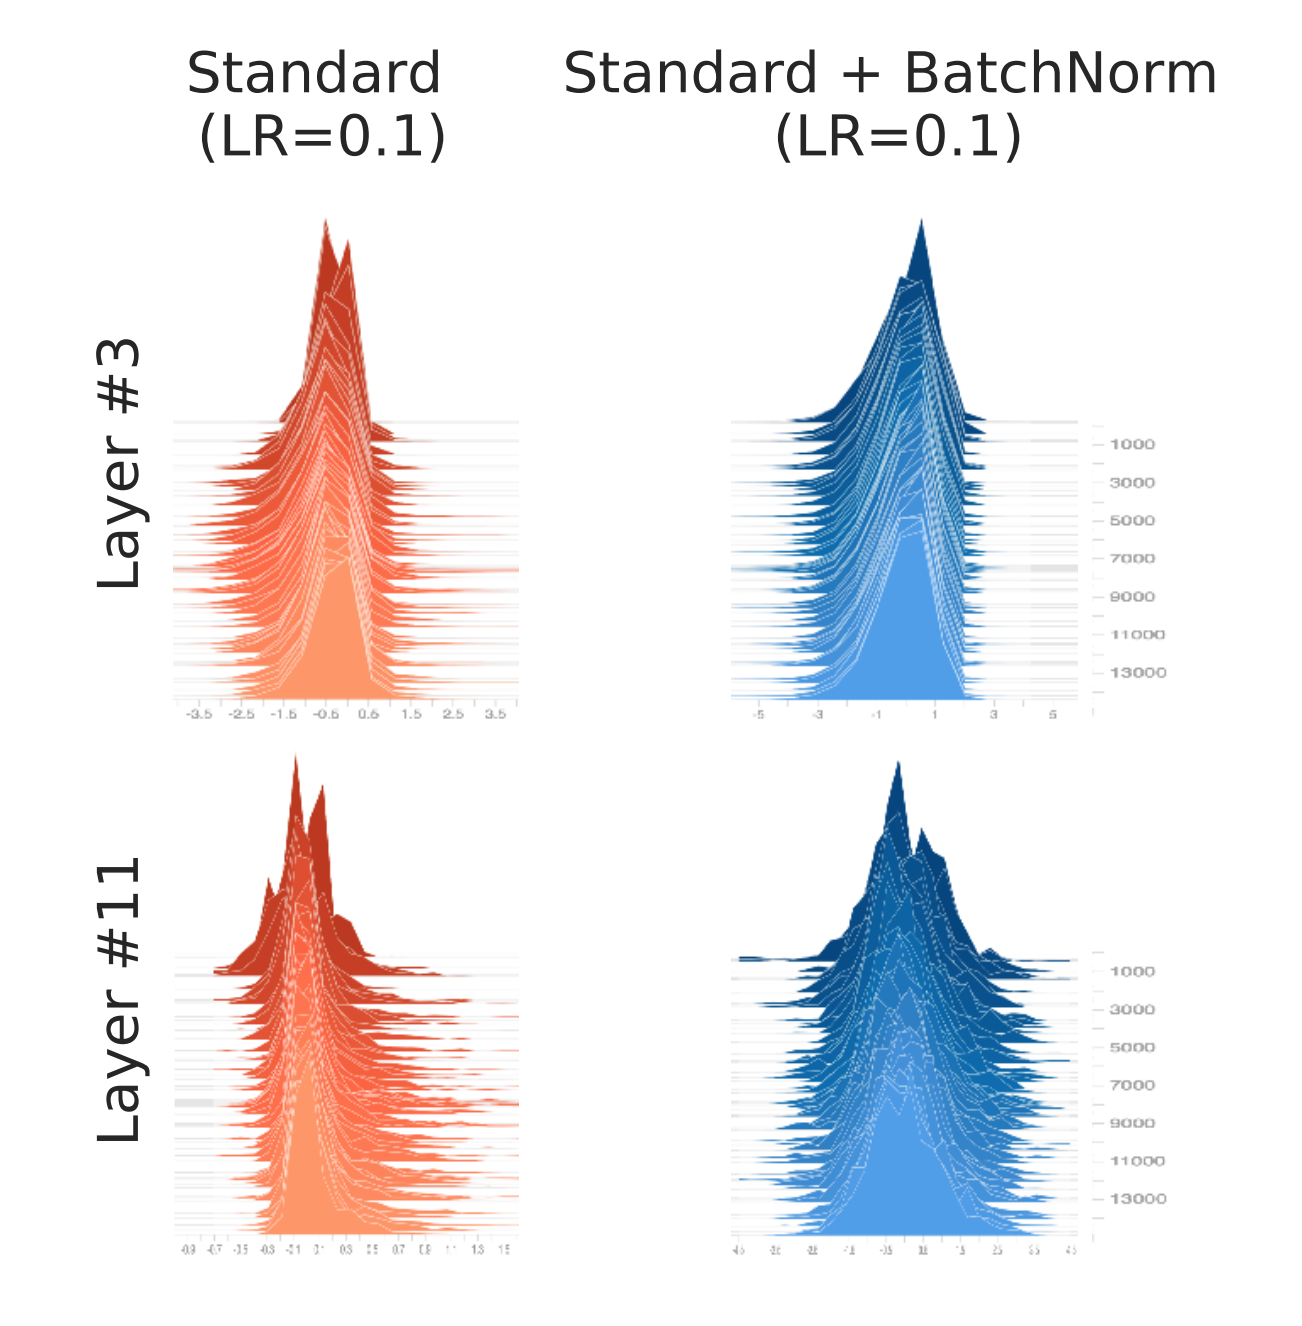
\includegraphics[width=.45\linewidth]{how_bn_help_2.png}
\end{center}
\vfill
\footnotesize
{\color{blue} \url{https://arxiv.org/abs/1805.11604}}
\end{frame}

\begin{frame}{Почему это помогает при обучении}
\begin{center}
	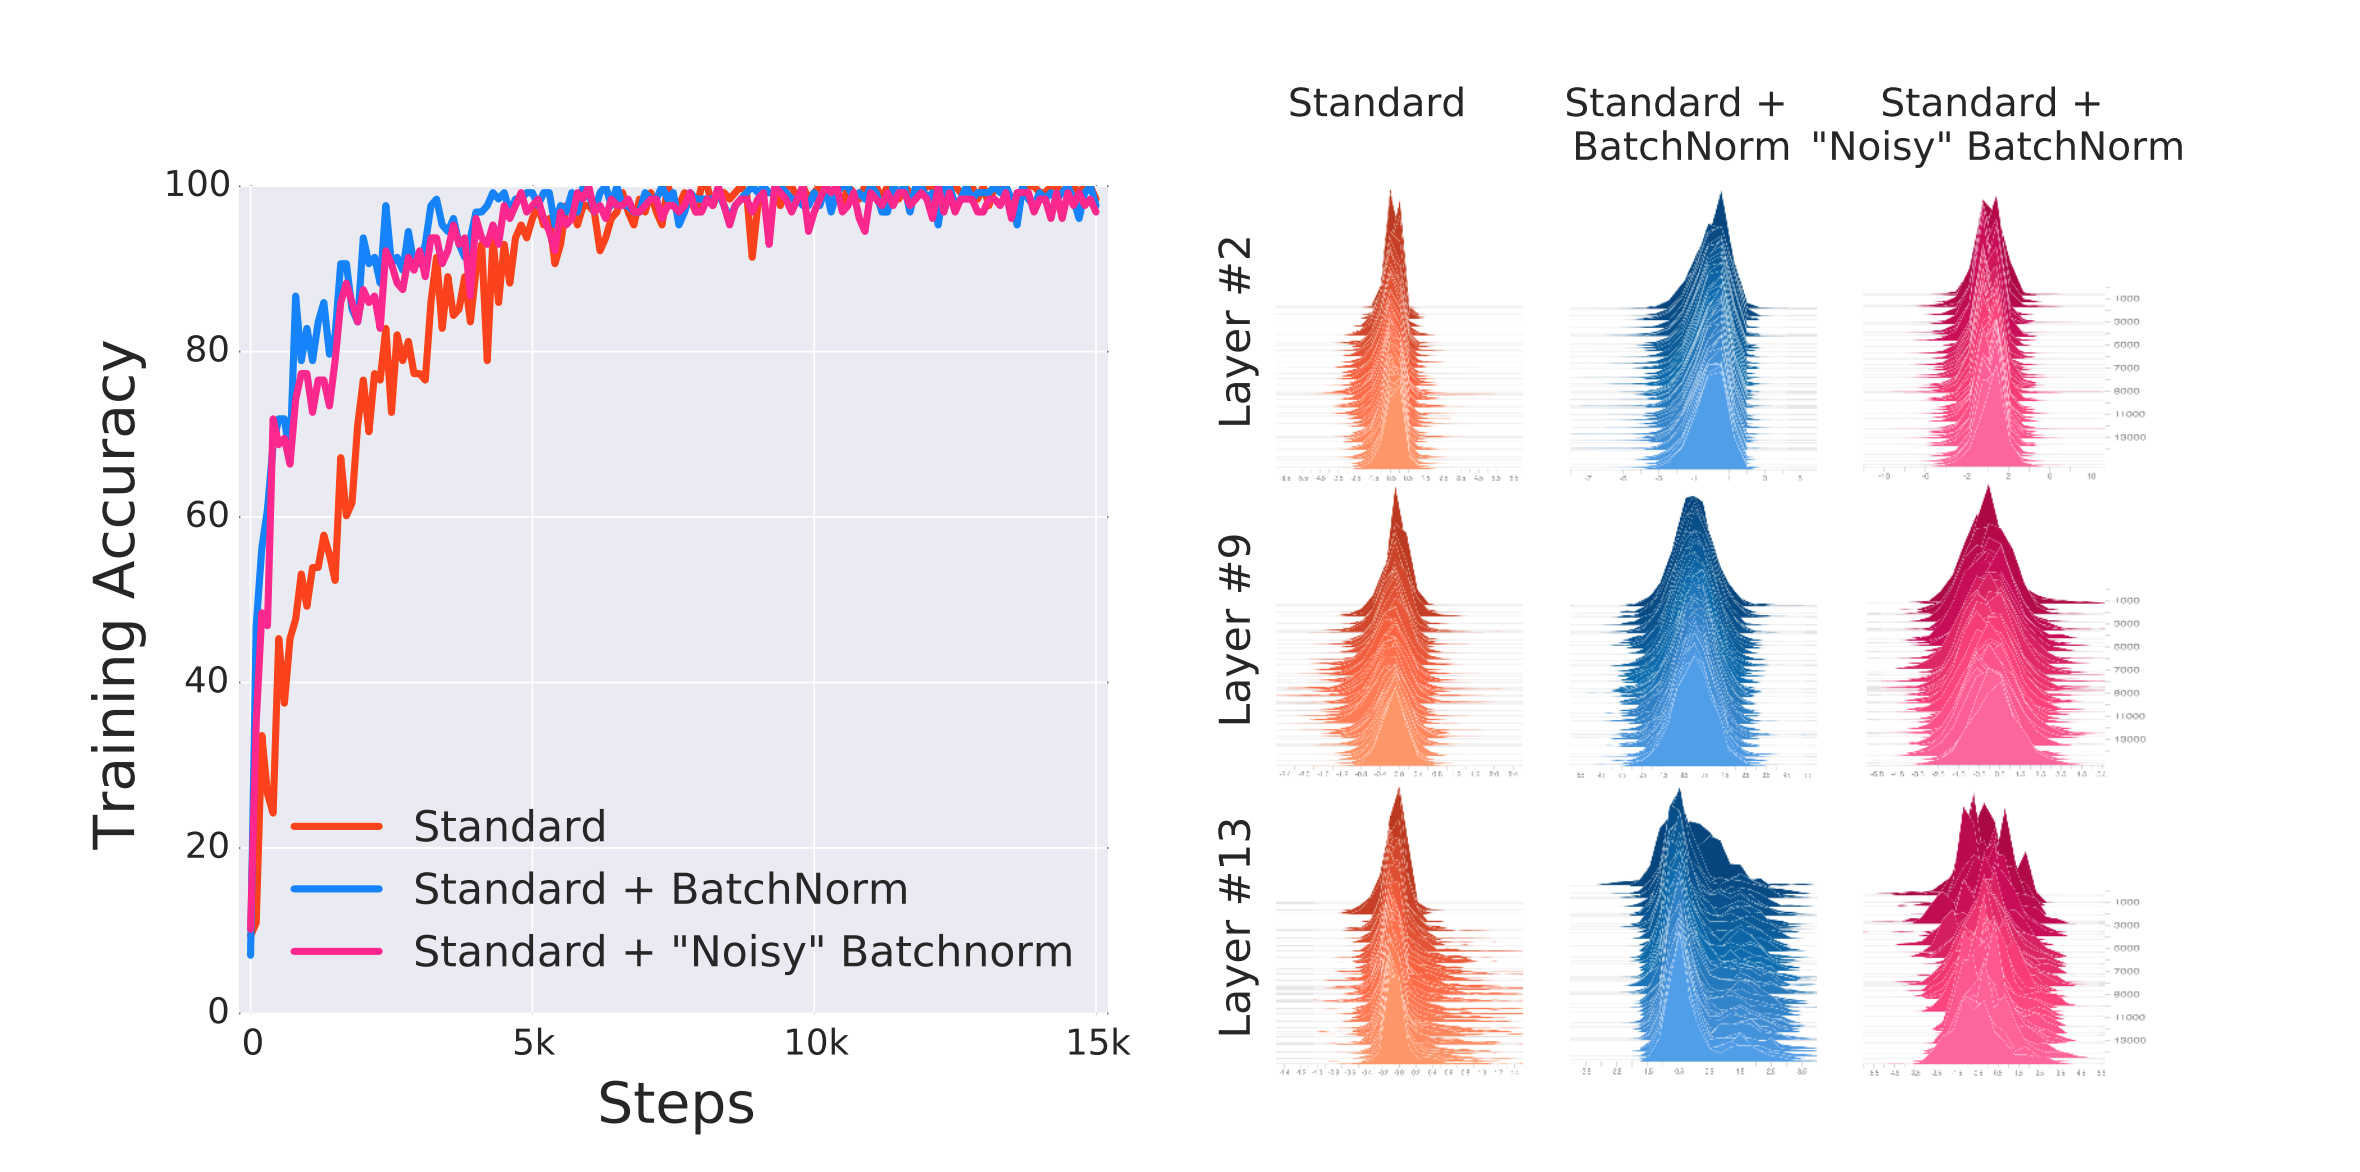
\includegraphics[width=.9\linewidth]{how_bn_help_3.png}
\end{center}
\vfill
\footnotesize
{\color{blue} \url{https://arxiv.org/abs/1805.11604}}
\end{frame}

\begin{frame}{Почему это помогает при обучении}
\alert{Батчнорм сглаживает ландшафт функции потерь и из-за этого градиентный спуск идёт более гладко.}
\begin{center}
	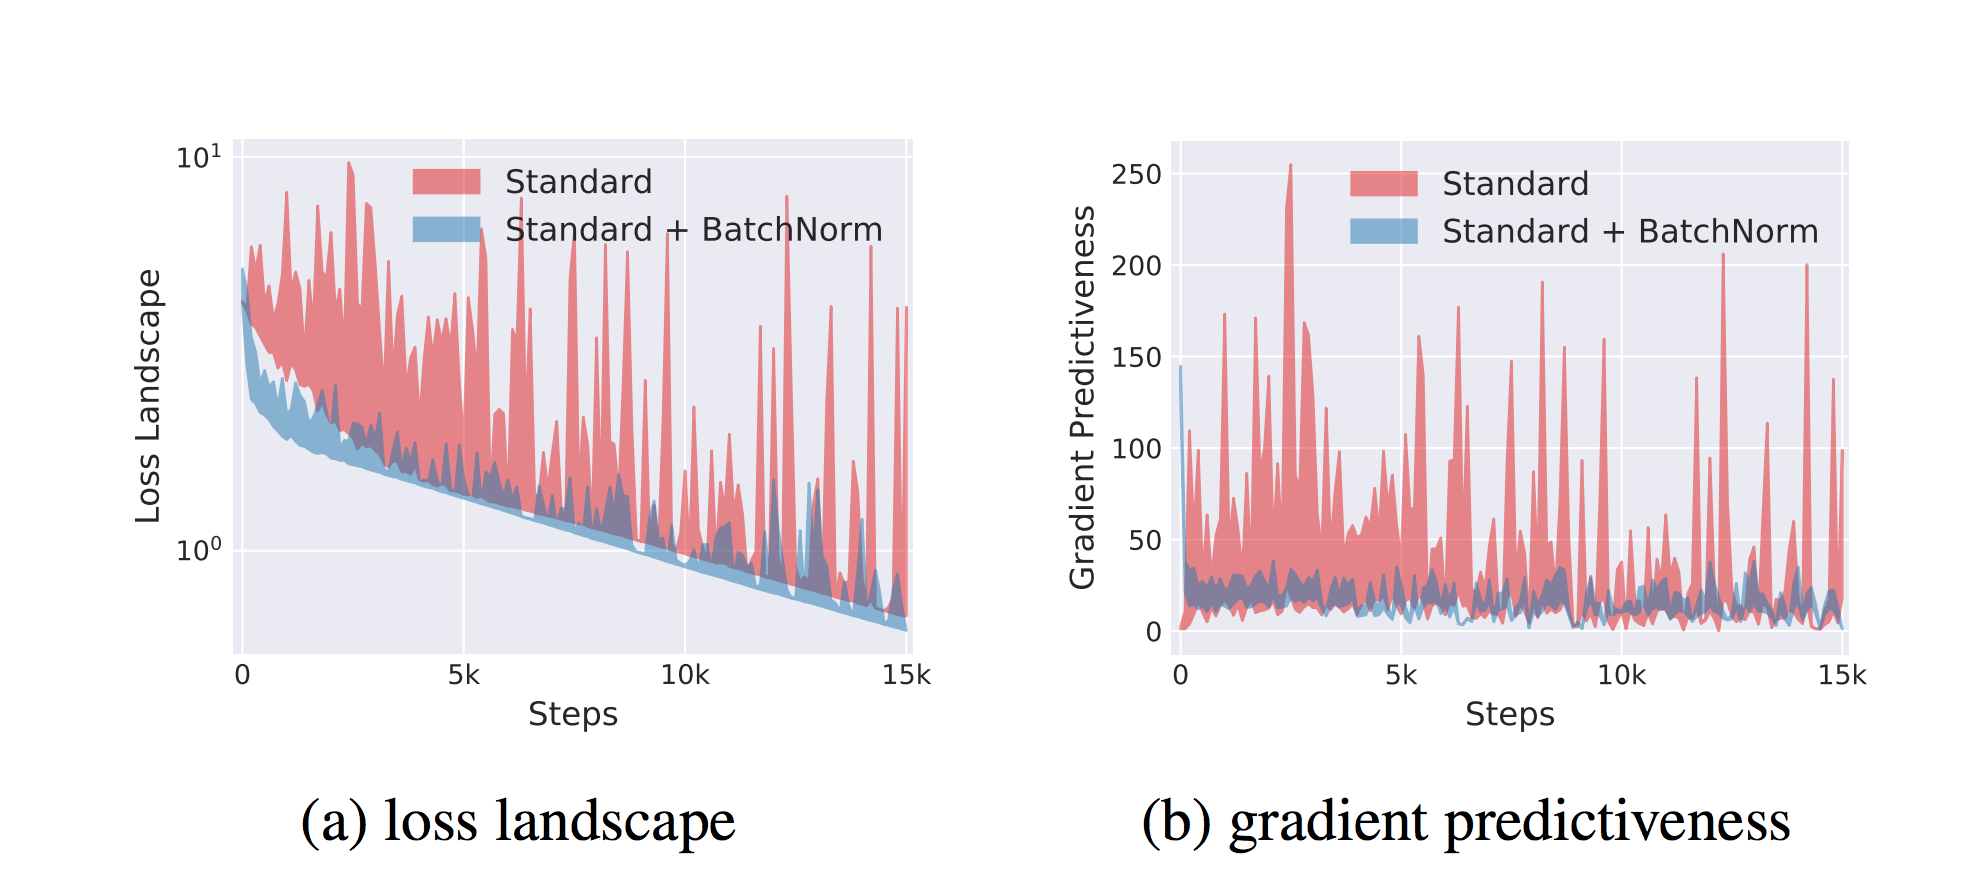
\includegraphics[width=.8\linewidth]{how_bn_help_4.png}
\end{center}
\vfill
\footnotesize
{\color{blue} \url{https://arxiv.org/abs/1805.11604}}
\end{frame}


\begin{frame}{Трюки}
\begin{wideitemize}
	\item  С батч-нормализацией нужно уменьшить силу Dropout и регуляризацию
	
	\item Батч-нормализация и Dropout могут конфликтовать 
	
	\item  Не забывайте перемешивать обучающую выборку перед каждой новой эпохой, чтобы батчи были разнообразными 
	
	\item Существует довольно много техник нормализации:  Layer Normalization, Weight Normalization, Batch Renormalization, Adaptive Instance Normalization, Group Normalization etc.	
\end{wideitemize}

\vspace{3cm} %
\footnotesize
{\color{blue} \url{http://openaccess.thecvf.com/content_CVPR_2019/papers/Li_Understanding_the_Disharmony_Between_Dropout_and_Batch_Normalization_by_Variance_CVPR_2019_paper.pdf}}
\end{frame}





\begin{transitionframe}
	\begin{center}
		\Huge  Инициализация весов
	\end{center}
	\centering 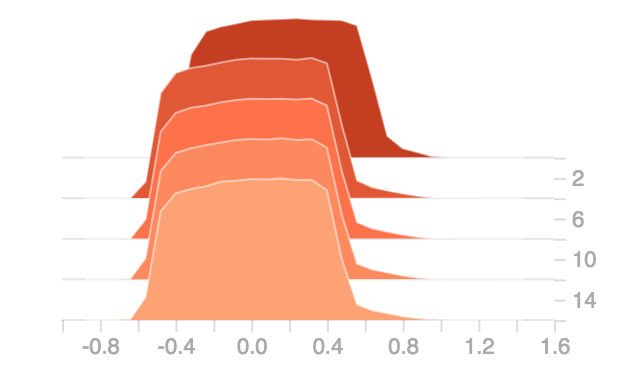
\includegraphics[scale = 0.2]{init.png}
\end{transitionframe}


\begin{frame}{Инициализация весов}
\begin{center}
	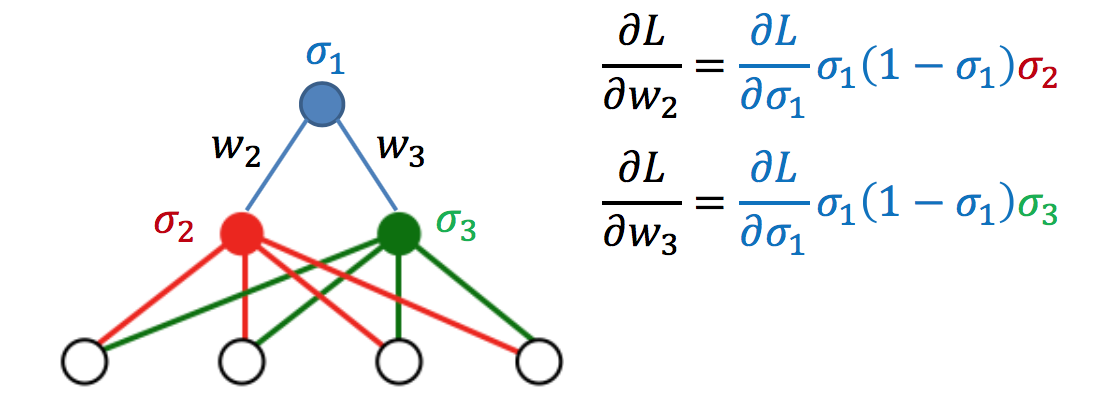
\includegraphics[width=.6\linewidth]{init1.png}
\end{center}
\begin{wideitemize}
	\item  Что будет, если инициализировать веса нулями?  \pause 
	\item  ${\color{red} \sigma_2 }$ и ${\color{green} \sigma_3 }$  будут обновляться одинаково
\end{wideitemize}
\end{frame}


\begin{frame}{Инициализация весов}
\begin{center}
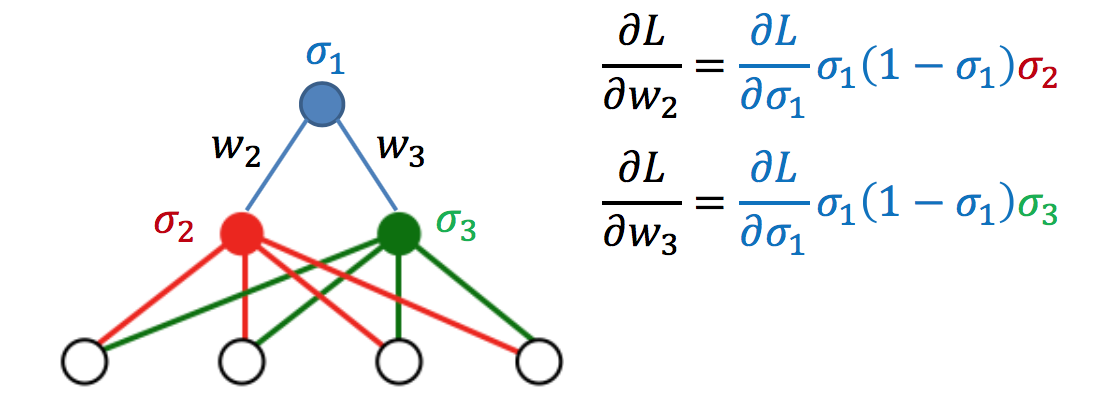
\includegraphics[width=.6\linewidth]{init1.png}
\end{center}
\begin{wideitemize}
\item  Хочется уничтожить симметрию
\item  Обычно инициализируют маленькими рандомными числами из какого-то распределения (нормальное, равномерное)
\end{wideitemize}
\end{frame}


\begin{frame}{Инициализация весов}
\begin{wideitemize}
\item Наши признаки $X$ пришли к нам из какого-то распределения 
\item Выход слоя $f(XW)$ будет принадлежать другому распределению 
\item Если инициализировать веса неправильно, дисперсия распределения може от слоя к слою затухать (сигнал будет теряться) либо наоброт, возрастать (сигнал будет рассеиваться)
\item Эмпирически было выяснено, что это может портить сходимость для глубоких сеток
\item  \alert{Хочется контролировать дисперсию} 
\end{wideitemize}
\end{frame}


\begin{frame}{Симметричный случай}
\begin{center}
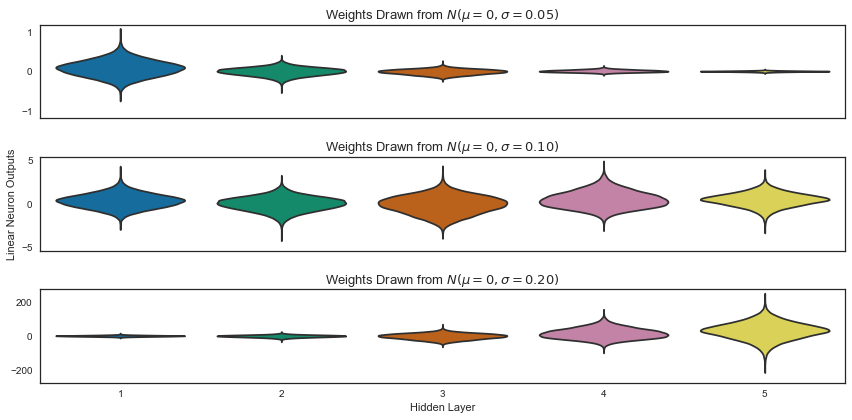
\includegraphics[width=.9\linewidth]{init_sim.png}
\end{center}
\end{frame}


\begin{frame}{Инициализация весов}
\begin{wideitemize}
\item  Посмотрим на выход нейрона перед активацией:
\begin{equation*}
\begin{aligned} 
h_i =  \sum_{i=1}^{n_{in}} w_i x_i 
\end{aligned}
\end{equation*}

\item  Дисперсия $h_i$ выражается через дисперсии $x$ и $w$ 

\item Будем считать, что веса $w_1, \ldots, w_k \sim iid$,  наблюдения $x_1, \ldots, x_n \sim iid$, а ещё $x_i$ и $w_i$ независимы между собой
\end{wideitemize}
\end{frame}

\begin{frame}{Инициализация весов (симметричный случай)}
\begin{multline*} 	
\Var(h_i) = \Var(\sum_{i=1}^{n_{in}} w_i x_i) =  \sum_{i=1}^{n_{in}} \Var(w_i x_i) = \\ 
= \sum_{i=1}^{n_{in}} [\E(x_i)]^2 \cdot \Var(w_i) + [\E(w_i)]^2 \cdot \Var(x_i)  + \Var(x_i) \cdot \Var(w_i)] = \only<3->{\\  =  \sum_{i=1}^{n_{in}}  \Var(x_i) \cdot \Var(w_i)  } \only<4>{ =  \Var(x)  \color{green} \cdot [n_{in} \cdot \Var(w)]} \only<5->{ =  \Var(x)  \color{green} \cdot \underbrace{[n_{in} \cdot \Var(w)]}_{= 1}}
\end{multline*}
\only<2-4>{

\begin{wideitemize}
\only<2>{ \item  Если функция активации симметричная, тогда $E(x_i) = 0$. Будем инициализировать веса с нулевым средним, тогда $E(w_i) = 0$.}

\only<3>{ 
\item  Предполагаем, что $x_i$ инициализируются из одного распределения, $w_i$ сами инициализируем из одного распределения.}

\only<4>{ 
\item  Хотим, чтобы зелёная штука была равна единице, тогда у потока будет всегда постоянная дисперсия, совпадающая с $\Var(x)$.}
\end{wideitemize}}

\only<1>{
\vfill %
\footnotesize
{\color{blue}  \url{https://en.wikipedia.org/wiki/Variance\#Product\_of\_independent\_variables}}}
\end{frame}


\begin{frame}{Плохая инициализация весов}
Пущай 

$$ w_i \sim U \left[ - \frac{1}{\sqrt{n_{in}}};  \frac{1}{\sqrt{n_{in}}}  \right],$$

тогда 

$$
\Var(w_i) = \frac{1}{12} \cdot \left( \frac{1}{\sqrt{n_{in}}} + \frac{1}{\sqrt{n_{in}}} \right)^2 = \frac{1}{3 n_{in}} \Rightarrow Var(h_i) = \frac{1}{3} 
$$

\alert{Получаем затухание!}
\end{frame}


\begin{frame}{Немного лучше}
Пущай 

$$ w_i \sim U \left[ - \frac{\sqrt{3}}{\sqrt{n_{in}}};  \frac{\sqrt{3}}{\sqrt{n_{in}}}  \right],$$

тогда 

$$
\Var(w_i) = \frac{1}{12} \cdot \left( \frac{\sqrt{3}}{\sqrt{n_{in}}} + \frac{\sqrt{3}}{\sqrt{n_{in}}} \right)^2 = \frac{1}{n_{in}} \Rightarrow Var(h_i) = 1 \pause 
$$

\vfill 
При forward pass на вход идёт $n_{in}$ набобдений, при backward pass на вход идёт $n_{out}$ градиентов $\Rightarrow$   \alert{канал с дисперсией может быть непостоянным, если число весов от слоя к слою сильно колеблется}
\end{frame}


\begin{frame}{Инициализация Ксавье (Глорота)}
Для неодинаковых размеров слоёв невозможно удволетворить обоим условиям, поэтому обычно усредняют и пытаются инициализировать веса с дисперсией $\frac{2}{n_{in} + n_{out}}$: 

$$ w_i \sim U \left[ - \frac{\sqrt{6}}{\sqrt{n_{out} + n_{in}}};  \frac{\sqrt{6}}{\sqrt{n_{out} + n_{in}}}  \right],$$

\vfill 

Такая инициализация называется \alert{инициализацией Ксавие (или Глорота)}

\vfill %
\footnotesize
{\color{blue} \url{http://proceedings.mlr.press/v9/glorot10a/glorot10a.pdf}}
\end{frame}


\begin{frame}{Несимметричный случай}
\begin{center}
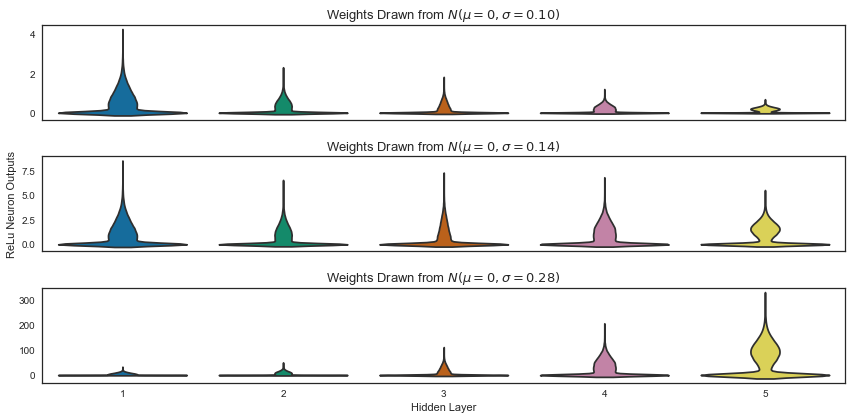
\includegraphics[width=.9\linewidth]{init_relu.png}
\end{center}
\end{frame}


\begin{frame}{Инициализация Хе}
\begin{multline*} 	
\Var(h_i) = \Var(\sum_{i=1}^{n_{in}} w_i x_i) =  \sum_{i=1}^{n_{in}} \Var(w_i x_i) = \\ 
= \sum_{i=1}^{n_{in}} [\E(x_i)]^2 \cdot \Var(w_i) + [\E(w_i)]^2 \cdot \Var(x_i)  + \Var(x_i) \cdot \Var(w_i)]  
\only<2->{= \\  = \sum_{i=1}^{n_{in}} [\E(x_i)]^2 \cdot \Var(w_i) +  \Var(x_i) \cdot \Var(w_i)  =  \sum_{i=1}^{n_{in}} \Var(w_i) \cdot E(x_i^2)} 
\only<3->{= \\  =  E(x^2)  \color{green} \cdot [n_{in} \cdot \Var(w)]}
\end{multline*}

\only<1-2>{	
\begin{wideitemize}
\item  Когда нет симметрии, можно занулить только второе слагаемое
\end{wideitemize}}
\end{frame}


\begin{frame}{Инициализация Хе}
\begin{align*} 	
\Var(h_i)  & =   E(x_i^2)  \cdot [n_{in} \cdot \Var(w)] \\
x_i & = \max(0; h_{i-1}) \\ 
\end{align*} \pause 

\only<2-> { Пусть $w_{i-1}$ распределены симметрично относительно нуля, тогда $h_{i-1}$ тоже будут симметрично распределены, тогда: }

$$
\only<3->{ E(x_i^2) = \frac{1}{2} \cdot \Var(h_{i-1}) }
$$

$$
\only<4->{ \Var(h_i) =  \frac{1}{2} \cdot \Var(h_{i-1}) \cdot [n_{in} \cdot \Var(w)]  \Rightarrow \Var(w_i) = \frac{2}{n_{in}} }
$$

\vfill %
\footnotesize
{\color{blue} \url{https://arxiv.org/pdf/1502.01852.pdf}}
\end{frame}


\begin{frame}{Кратикие итоги}
\begin{wideitemize}
\item  Для симметричных функций с нулевым средним используйте инициализацию Ксавье (Глорота) {\color{green}  init="glorot\_uniform"} 
\item  Для ReLU и им подобным инициализацию Хe {\color{green} init="he\_uniform"} или {\color{green} init="he\_nomal"}
\item  Эти две инициализации корректируют параметры распределений в зависимости от входа и выхода слоя так, чтобы поддерживать дисперсию равной единице
\end{wideitemize}
\end{frame}


\begin{frame}{Эксперимент с MNIST}
\begin{center}
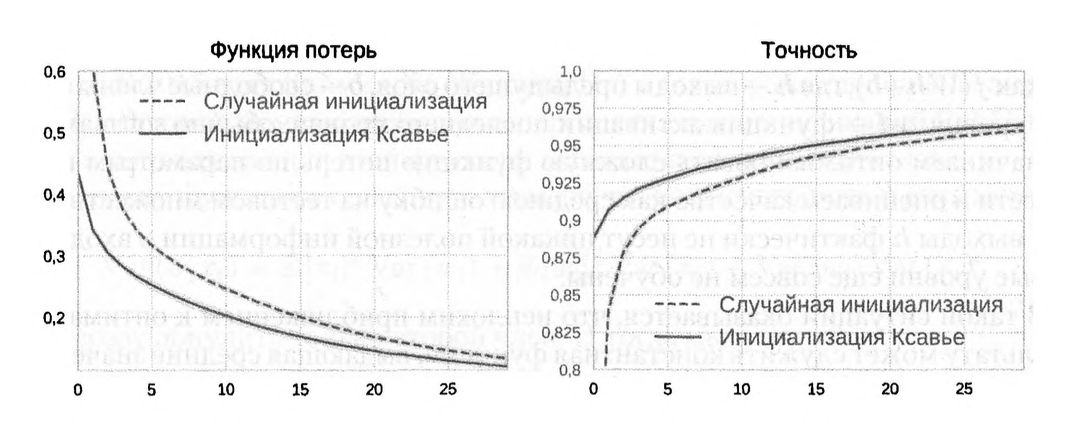
\includegraphics[width=.8\linewidth]{nicol_init.png}
\end{center}

\vfill
{\small  Источник: Николенко, страница 149}
\end{frame}





\begin{transitionframe}
	\begin{center}
		% \Huge Dropout  
		
\includegraphics[scale = 0.3]{dropout_beer.png}
	\end{center}
\end{transitionframe}

{
	\usebackgroundtemplate{ 
		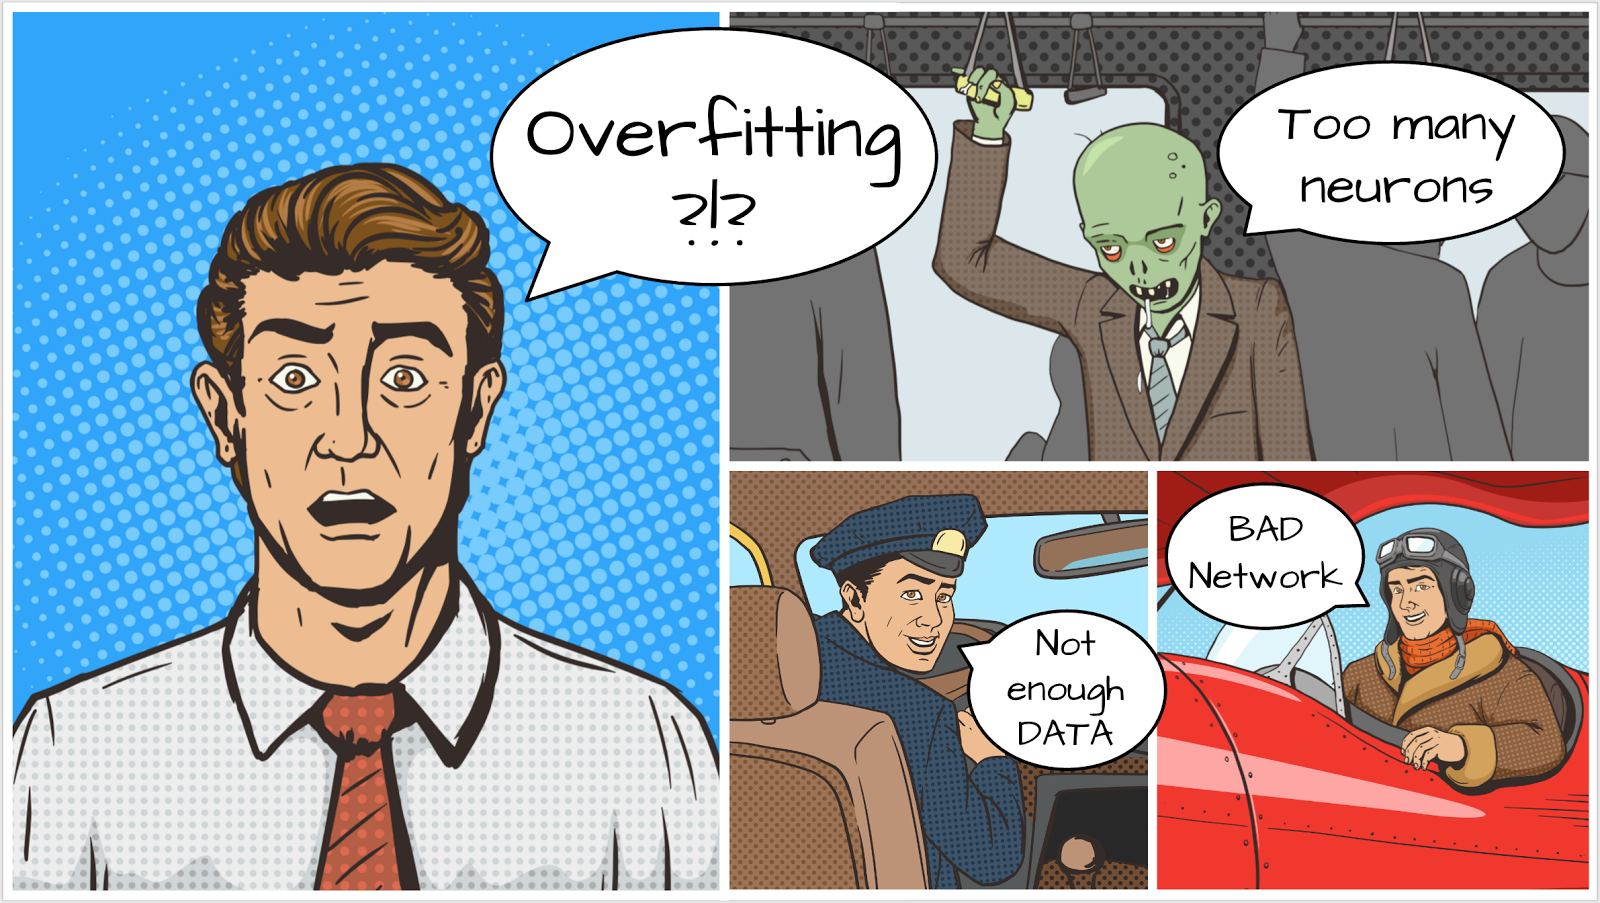
\includegraphics[width=\paperwidth]{overfitting.png}}
	\begin{frame}
\end{frame}
}

\begin{frame}{Dropout}
\begin{wideitemize}	
	\item Оставляем нейрон с вероятностью $p$, иначе отключаем (заменяем на $0$)
	
	\item Делает нейроны более устойчивыми к случайным возмущениям
	
	\item Борьба с ко-адоптацией, не все соседи похожи, не все дети похожи на родителей
\end{wideitemize}

\begin{center}
	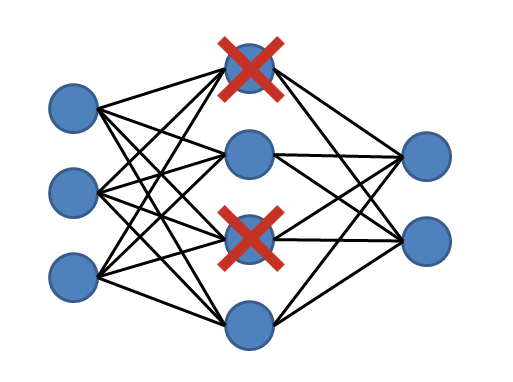
\includegraphics[width=.35\linewidth]{dropout.png}
\end{center}

\vfill %
\footnotesize
{\color{blue} \url{http://www.cs.toronto.edu/~rsalakhu/papers/srivastava14a.pdf}}
\end{frame}


\begin{frame}{Dropout в формулах} 
	\begin{wideitemize}
		\item 	\alert{forward pass:} 
		
		\begin{equation*}
			\begin{aligned}
			& o = f(X \cdot W + b ) \\
			\only<2->{ & \alert{o = D \cdot f(X \cdot W + b ), \quad  D = (D_1, \ldots, D_k) \sim iid \vspace{5mm} Bern(p) } }
			\end{aligned}
		\end{equation*}
		
		\only<3>{
		\vfill
		$$
		o_i = D_i \cdot f(w x_i^T + b) = \begin{cases} f(w x_i^T + b) , 1-p \\ 0, p \end{cases}
		$$
		\vfill 
		Дропаут — это просто небольшая модификация функции активации
		}
\vfill
		\only<4->{
		\item  	\alert{backward pass:} 
		\begin{equation*}
			\begin{aligned}
			& d = f'(h) \cdot W \cdot d  \\
			& \alert{ d =  D \cdot f'(h) \cdot W \cdot d} 
			\end{aligned}
		\end{equation*}			
		}	
	\end{wideitemize}
\end{frame}


\begin{frame}{Dropout}
\begin{wideitemize}
\item  При обучении мы домножаем часть выходов на $D_i$, тем самым мы изменяем только часть параметров и нейроны учатся более независимо  $\Rightarrow$ регуляризация

\item  Dropout эквивалентен обучению $2^n$ сетей

\only<1>{
\begin{center}
	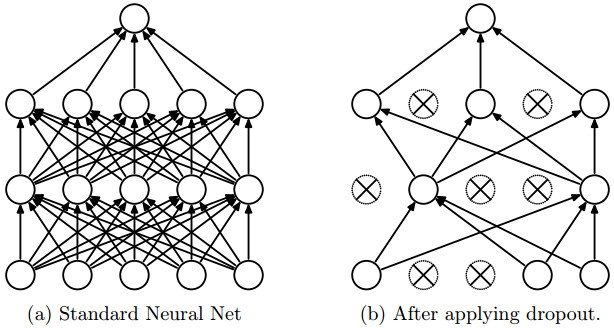
\includegraphics[width=0.5\paperwidth]{dropout2.png}
\end{center} }

\only<2>{\alert{ \item  Что делать на стадии тестирования?}}

 \only<3->{
\item Нам надо сымитировать работу такого ансамбля: можно отключать по очереди все возможные комбинации нейронов, получить $2^n$ прогнозов и усреднить их }

 \only<4->{ \item Но лучше просто брать по дропауту математическое ожидание 

$$
o = p \cdot f(X \cdot W + b)
$$}
\end{wideitemize}
\end{frame}


\begin{frame}{Обратный Dropout}
\begin{wideitemize}
	\item   На тесте ищем математическое ожидание: 
		$$
		o = p \cdot f(X \cdot W + b)
		$$ \pause
		
	\item \alert{Это неудобно! Надо переписывать функцию для прогнозов!}  \pause
	
	\item Давайте лучше будем домножать на $\frac{1}{p}$ на этапе обучения: 
	
	\begin{equation*}
		\begin{aligned}
			& \alert{ \text{train: }}  o = \frac{1}{p} \cdot D \cdot f(X \cdot W + b) \\ 
			& \alert{\text{test:  }}   o = f(X \cdot W + b) \\
		\end{aligned}
	\end{equation*}		
\end{wideitemize}
\end{frame}

%В стандартной нейронной сети производная, полученная каждым параметром, сообщает ему, как он должен измениться, чтобы, учитывая деятельность остальных блоков, минимизировать функцию конечных потерь. Поэтому блоки могут меняться, исправляя при этом ошибки других блоковкарпатый dropout. Это может привести к чрезмерной совместной адаптации (co-adaptation), что, в свою очередь, приводит к переобучению, поскольку эти совместные адаптации невозможно обобщить на данные, не участвовавшие в обучении. Мы выдвигаем гипотезу, что Dropout предотвращает совместную адаптацию для каждого скрытого блока, делая присутствие других скрытых блоков ненадежным. Поэтому скрытый блок не может полагаться на другие блоки в исправлении собственных ошибок.

%Dropout хорошо работает на практике, потому что предотвращает взаимоадаптацию нейронов на этапе обучения.

\begin{transitionframe}
		\centering 
\includegraphics[scale = 0.25]{eto-drugoe.png}
	\begin{center}
		\Huge  Другая регуляризация
	\end{center}
\end{transitionframe}

\begin{frame}{Уже обсуждали}
\begin{wideitemize}
	\item $l_1$ и $l_2$ регуляризация 
	\item Ранняя остановка 
	\item Различные новые градиентные спуски, ускоряющие процедуру сходимости 
\end{wideitemize}
\end{frame}

\begin{frame}{Early stopping}
\begin{center}
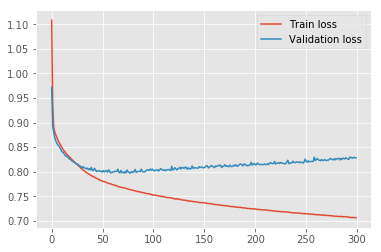
\includegraphics[width=0.5\paperwidth]{early_stopping.png}
\end{center}
\begin{wideitemize}
\item Будем останавливать обучение, когда качество на валидации начинает падать
\end{wideitemize}
\end{frame}

\begin{frame}{Регуляризация}
\begin{wideitemize}
\item $L_2$: приплюсовываем к функции потерь $\lambda \cdot \sum w_i^2$

\item $L_1$: приплюсовываем к функции потерь $\lambda \cdot \sum |w_i|$

\item Можно регуляризовать не всю сетку, а отдельный нейрон или слой 

\item Не даёт нейрону сфокусироваться на слишком выделяющемся входе	
\end{wideitemize}
\end{frame}


\begin{frame}{Регуляризация}
\begin{wideitemize}
\item В keras можно добавить для каждого слоя на три вида связей: 

\item \textbf{kernel\_regulirizer} - на матрицу весов слоя;

\item \textbf{bias\_regulirizer} - на вектор свободных членов;

\item \textbf{kernel\_regulirizer} - на вектор выходов.

\item \textbf{Делается примерно так:}

\mbox{ }

\pgr{\hspace{50pt}} model.add(Dense(256, inpit\_dim = 32, \\
\pgr{\hspace{80pt}}  kernel\_regulirizer = regulizers.l1(0.001), \\
\pgr{\hspace{80pt}} bias\_regulirizer = regulizers.l2(0.1), \\
\pgr{\hspace{80pt}} activity\_regulirizer = regulizers.l2(0.01))) 
\end{wideitemize}
\end{frame}


\begin{frame}{Взаимосвязи}
\begin{wideitemize}
\item  На практике обычно используют Dropout. Действия всех этих регуляризаторов оказывается схожим: 

\item Например, в [1] написано: \\ \mbox{   } \\

\texttt{«We show that the dropout regularizer is first-order equivalent to an L2 regularizer applied after scaling the features by an estimate of the inverse diagonal Fisher information matrix»}

\item  У Гудфеллоу в Глубоком обучении на стр. 218 можно найти, что рання остановка для линейных моделей эквивалентна $l_2$ регуляризации с MSE, обучаемой SGD.

\end{wideitemize}

\vfill %
\footnotesize 
\color{blue} [1] \url{https://arxiv.org/abs/1307.1493} 
\end{frame}


%%%%%%%  В презу с эвристиками ! 

\begin{frame}{Размеры сеток и переобучение}
\begin{center}
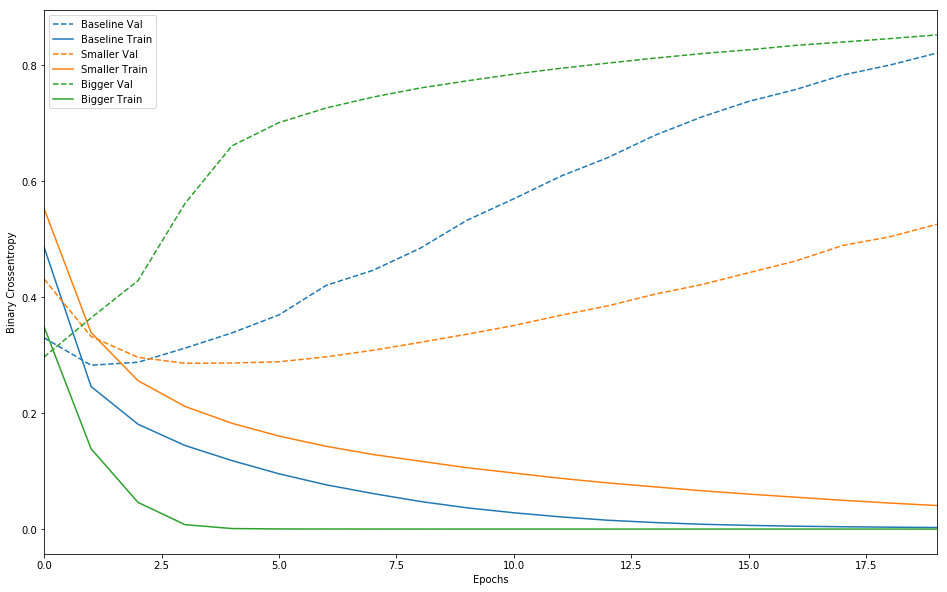
\includegraphics[width=0.7\paperwidth]{big_base_small_fit.png}
\end{center}
\end{frame}


\begin{frame}{Предобучение}
\begin{wideitemize}
	\item  Обучаем каждый нейрон на рандомной подвыборке, каждый нейрон впитает какие-то отдельные её особенности, после скрепляем все нейроны вместе и продолжаем обучение на всей выборке
	
	\item  \alert{На будущее:} обучаем на корпусе картинок автокодировщик, encoder благодаря этому учится выделять наиболее важные фичи, которые позволяют эффективно сжимать изображения. После срезаем decoder и на его месте достраиваем слои для решения нашей задаче, запускаем обычное дообучение.
\end{wideitemize}
\end{frame}


\begin{frame}{Динамическое наращивание сети}
\begin{wideitemize}
\item  Обучение сети при заведомо недостаточном числе нейронов $H$
\item После стабилизации функции потерь — добавление нового нейрона и его инициализация путём обучения 
\begin{itemize}
	\item либо по случайной подвыборке 
	\item либо по объектам с наибольшими значениями потерь 
	\item либо по случайному подмножеству входов
	\item либо из различных случайных начальных приближений
\end{itemize}
\item Снова итерации BackProp
\end{wideitemize}

\vfill
\begin{center}
\alert{Эмпирический опыт:} Общее время обучения обычно лишь в $1.5-2$ раза больше, чем если бы в сети сразу было итоговое число нейронов. Полезная информация, накопленная сетью не теряется при добавлении нейронов.
\end{center}
\end{frame}


\begin{frame}{Прореживание сети}
\begin{wideitemize}
\item Начать с большого количество нейронов и удалять незначимые по какому-нибудь критерию 
\item \alert{Пример:} обнуляем вес, смотрим как сильно упала ошибка, сортируем все cвязи по этому критерию, удаляем $N$ наименее значимых
\item После прореживания снова запускаем backprop
\item Если качество модели сильно упала, надо вернуть последние удалённые связи 
\end{wideitemize}
\end{frame}


\begin{transitionframe}
	\begin{center}
		\Huge  Skip-connection и ResNet
	\end{center}
	\centering 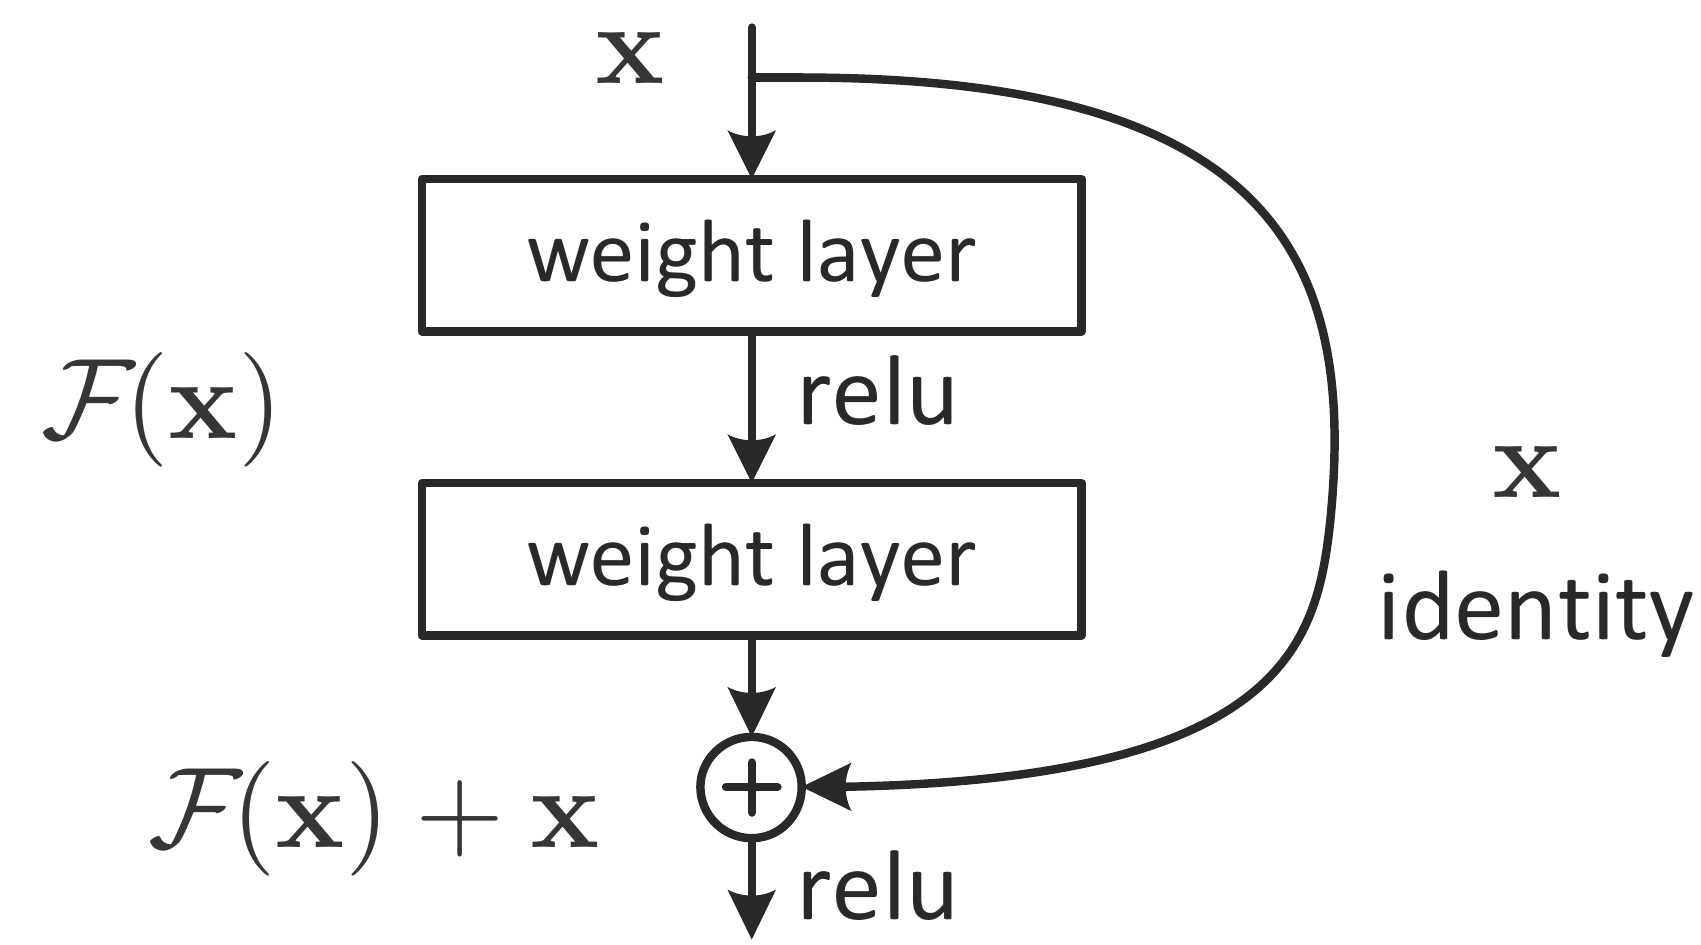
\includegraphics[scale = 0.1]{resnet_layer.png}
\end{transitionframe}

\begin{frame}{Очень глубокие сети}
\begin{center}
	
\includegraphics[width=0.8\paperwidth]{we-need-to-go-deeper.jpg}
\end{center}
\end{frame}


\begin{frame}{Идея ResNet}

Чем глубже нейронная сеть, тем сложнее её обучать, возникает новая проблема, которую нельзя свести к переобучению или затуханию градиента. \alert{Её называют деградация обучения (training degradation)}

\begin{center}
	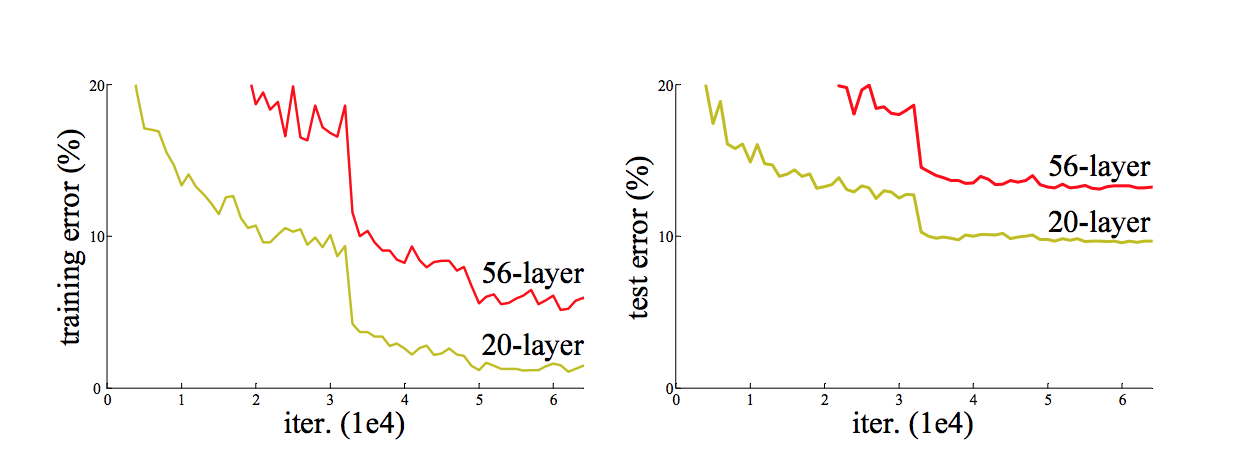
\includegraphics[width=0.8\paperwidth]{resnet_idea.png}
\end{center}

\vfill %
\footnotesize
\color{blue} \url{https://arxiv.org/abs/1512.03385}
\end{frame}

\begin{frame}{Идея ResNet}
\begin{wideitemize}
	\item  Огромная свёрточная сеть из $20$ слоёв и свёрточная сеть из $56$ слоёв,  большая сетка обучается хуже
	\item  \alert{Проблема:} слои инициализированы шумом, если какой-то один слой не натренирован, он убивает работу сети, через него не проходит полезный сигнал 
	\item Чем больше слоёв, тем более ярко выражен этот эффект 
	\item \alert{Решение:} Будем посылать вход на выход и давать слою возможность немного его подправить (residual слой)
	\item Идея чем-то похожа на бустинг, сеть сама решает когда заканчивать подправлять выходы (грубо говоря, сама выбирает глубину)
\end{wideitemize}
\end{frame}


\begin{frame}{ResNet (2015)}
\begin{center}
	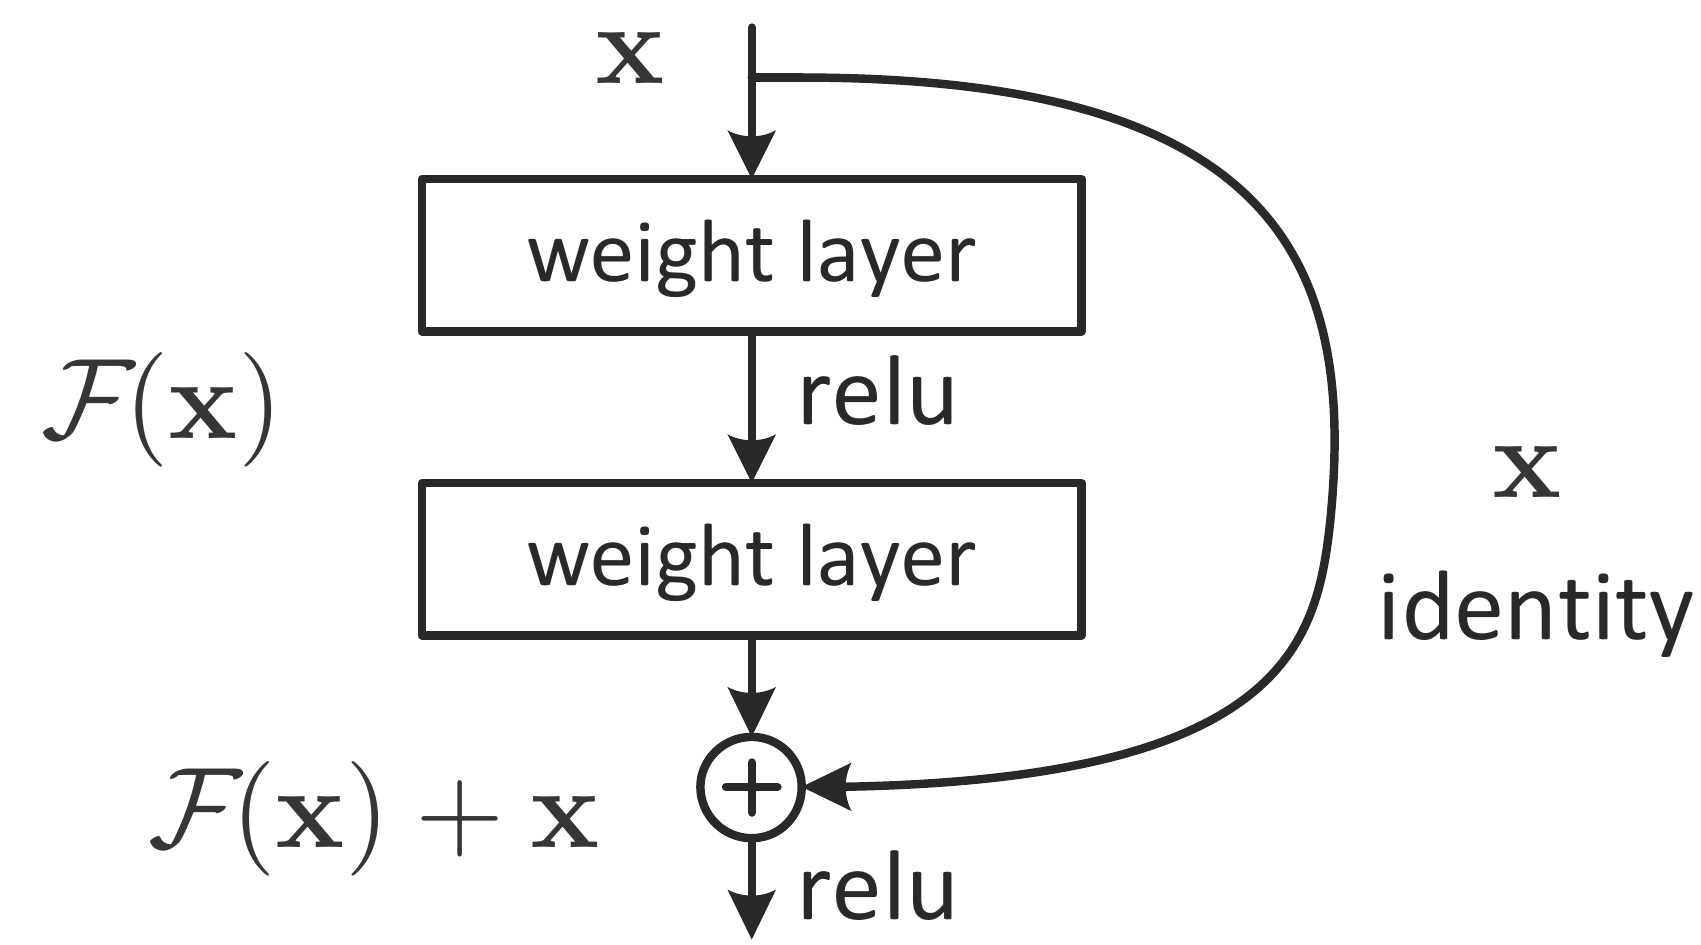
\includegraphics[scale=0.2]{resnet_layer.png}
\end{center}
\vfill %
\footnotesize
\color{blue} \url{https://arxiv.org/abs/1512.03385}
\end{frame}


\begin{frame}{ResNet (2015)}
\begin{center}
	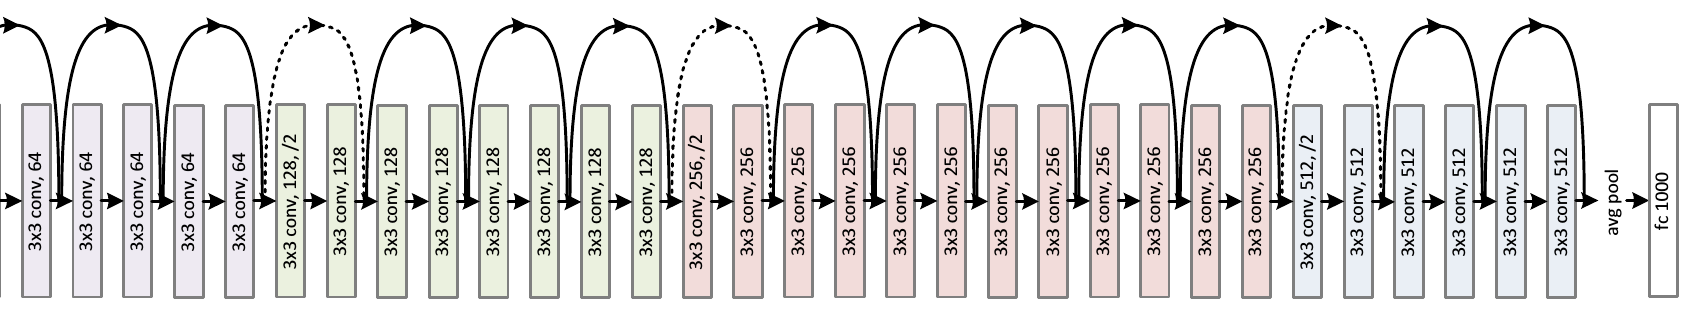
\includegraphics[width=0.8\paperwidth]{resnet.png}
\end{center}
\vfill %
\footnotesize
\color{blue} \url{https://arxiv.org/abs/1512.03385}
\end{frame}


\begin{frame}{ResNet (2015)}
\begin{wideitemize}
\item \alert{Идея:} более глубокие уровни должны улавливать разницу между новым и тем, что было раньше 

\item Ключевым элементом архитектуры является связь, которая пропускает несколько слоёв, передавая результат предыдущего слоя

\item Такое изменение позволило полностью отказаться от таких техник регуляризации, как DropOut

\item Градиенты не взрываются, свойства ResNet активно пытаются сейчас изучать

\item  ResNet-архитектура ведёт себя как ансамбль неглубоких сетей:  \color{blue} \url{https://arxiv.org/abs/1605.06431}
\end{wideitemize}
\end{frame}


\begin{frame}{Визуализация потерь}
\begin{center}
	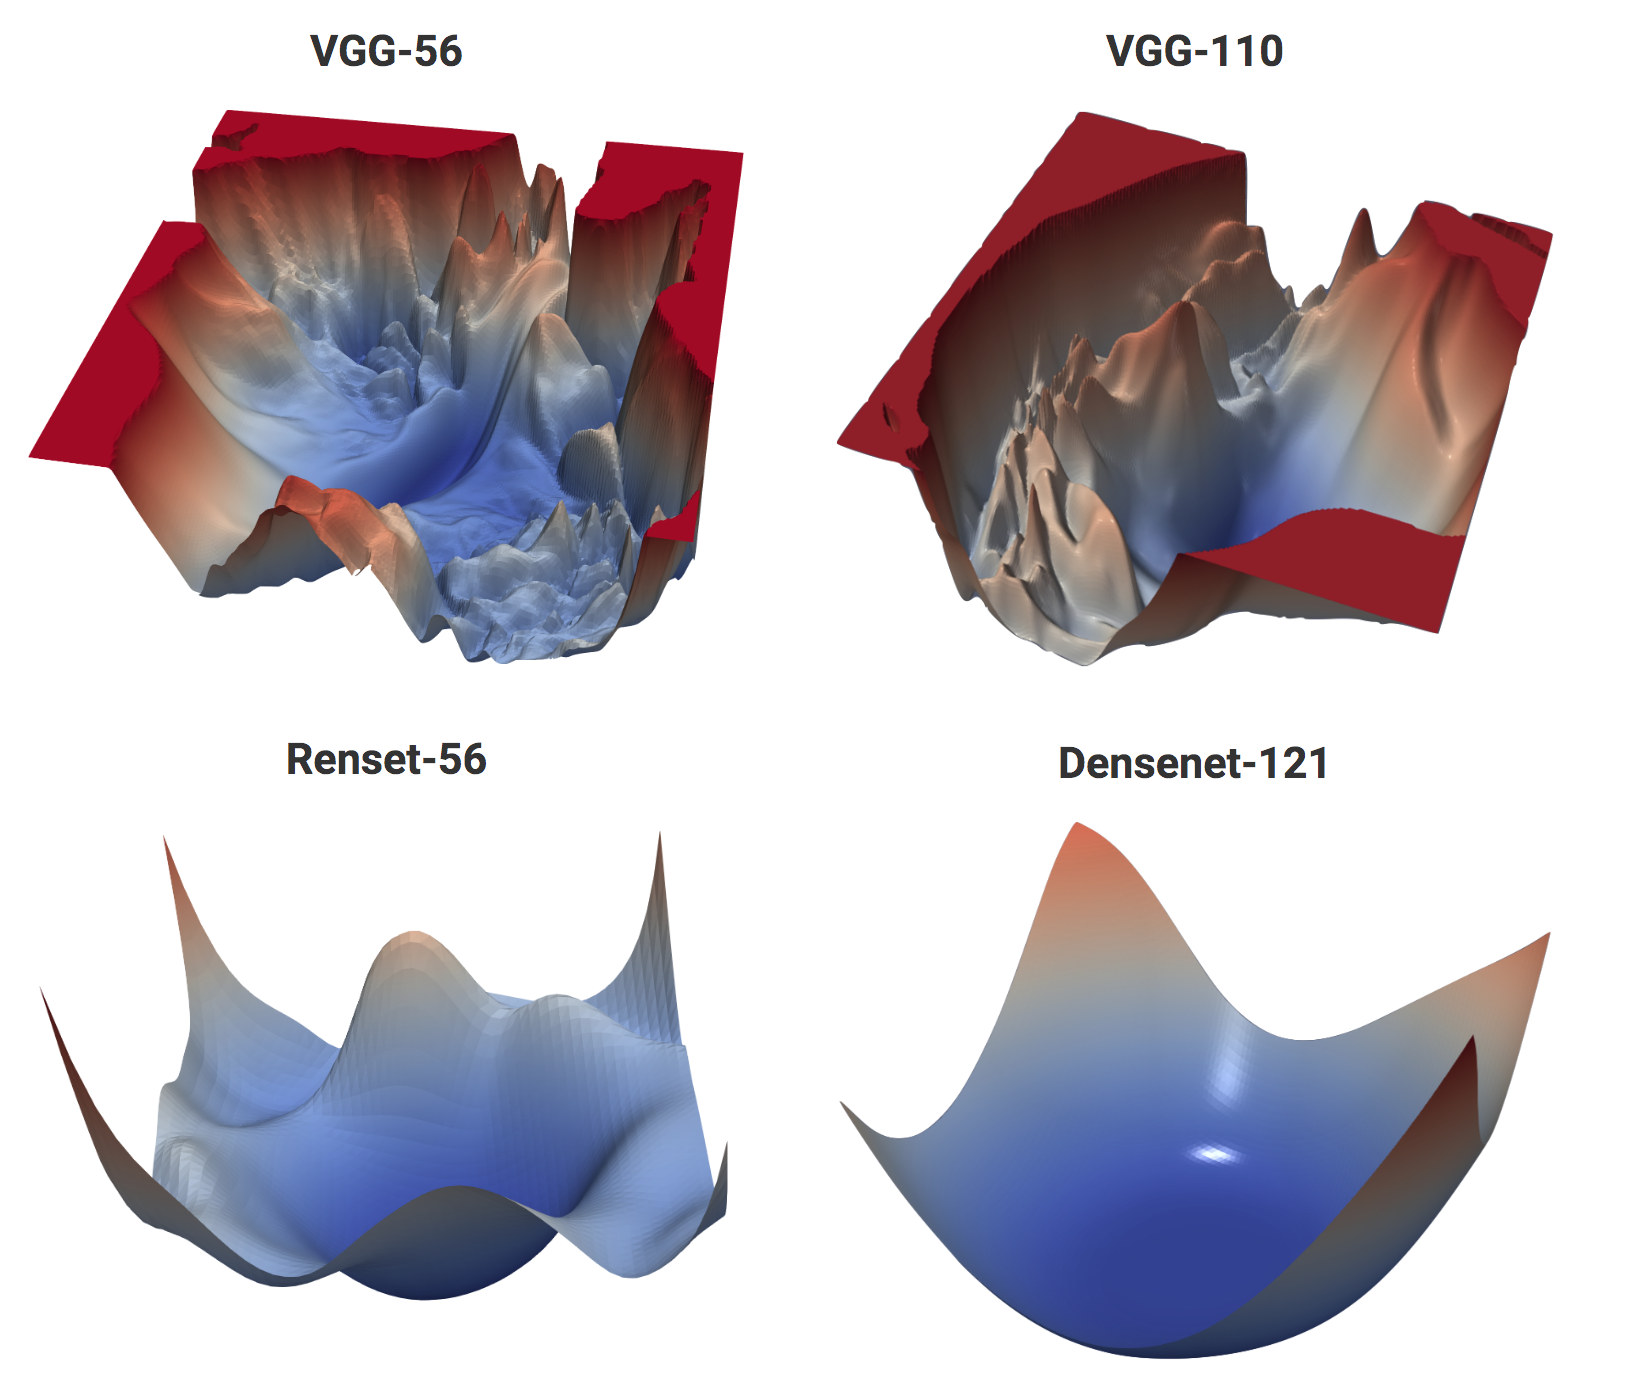
\includegraphics[width=0.5\paperwidth]{loss.png}
\end{center}
\vfill %
\footnotesize 
\color{blue} \url{https://arxiv.org/pdf/1712.09913.pdf} \newline  \url{https://github.com/tomgoldstein/loss-landscape}
\end{frame}


\begin{frame}{ResNet}
\begin{wideitemize}
	\item  ResNet породил целый букет новых архитектур
	
	\item Сегодня эта идея активно используется в рекурентных сетках и трансформерах 
\end{wideitemize}
\end{frame}


\begin{transitionframe}
	\begin{center}
		\Huge  Нейросети со стохастической глубиной
	\end{center}
	\centering 
\includegraphics[scale = 0.1]{deep.png}
\end{transitionframe}


\begin{frame}{Нейросети со стохастической глубиной}
\begin{center}
	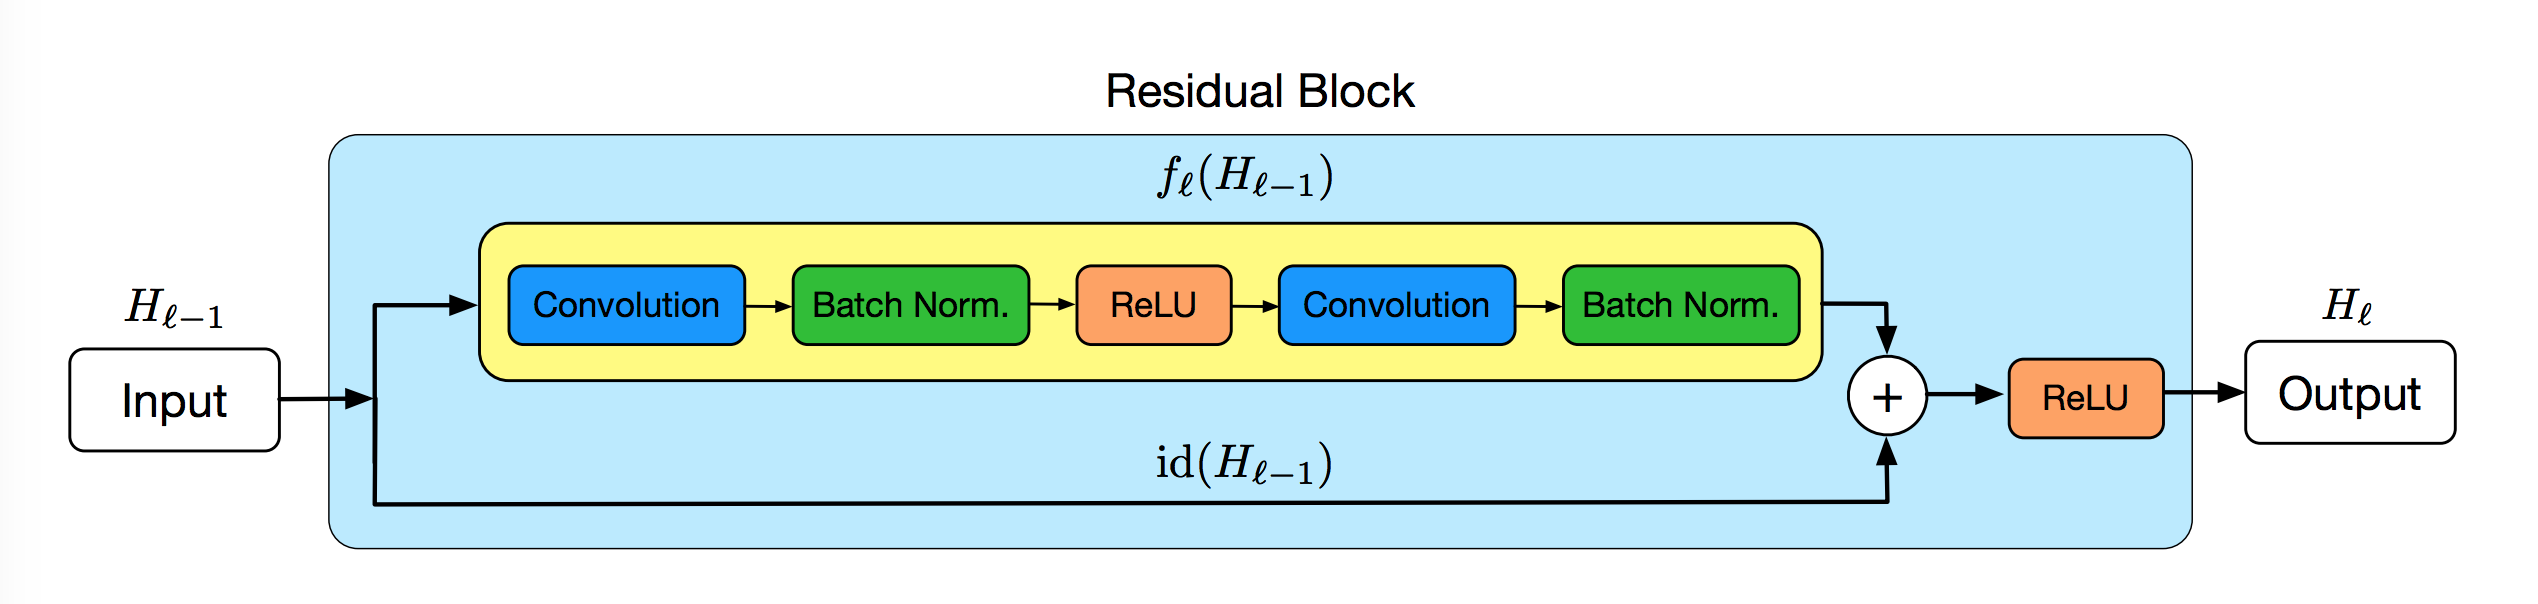
\includegraphics[width=0.9\paperwidth]{resnet_stoc.png}
\end{center}

Обычный RESNET-блок: 

\[
H_l = ReLU(f_l(H_{l-1}) + H_{l-1} ) 
\]

\vfill %
\footnotesize 
\color{blue} \url{https://arxiv.org/abs/1603.09382}
\end{frame}


\begin{frame}{Нейросети со стохастической глубиной}
\begin{center}
	\includegraphics[width=0.9\paperwidth]{resnet_stoc.png}
\end{center}

Немного видоизменим его: 

\begin{equation*}
\begin{aligned}
& b_l \sim Bern(p_l) \\
& H_l = ReLU(b_l \cdot f_l(H_{l-1}) + H_{l-1} ) 
\end{aligned} 
\end{equation*}

\vfill %
\footnotesize 
\color{blue} \url{https://arxiv.org/abs/1603.09382}
\end{frame}


\begin{frame}{Нейросети со стохастической глубиной}
\begin{wideitemize}
	\item  Для слоя $l$ мы задаём вероятность $p_l$, которая сохраняет этой слой в нейронной сетке
	
	\item Если $b_l = 1$, у нас остаётся обычный RESNET-блок, если $b_l = 0$ остаётся только skip-connection
	
	\item Глубина сетки зависит от того, как сгенирируется случайная величина
	
	\item Как подобрать $p_l$? 
	
	\item Первые слои важнее, так как они создают скрытые представления
\end{wideitemize}
\end{frame}


\begin{frame}{Нейросети со стохастической глубиной}

\[
p_l = 1 - \frac{l}{L} \cdot (1 - p_L), \quad p_L = const \in [0;1]
\]

\begin{center}
	\includegraphics[width=0.9\paperwidth]{save_resnet.png}
\end{center}

\vfill %
\footnotesize 
\color{blue} \url{https://arxiv.org/abs/1603.09382}
\end{frame}


\begin{frame}{Этап предсказания}
\begin{center}
	\includegraphics[width=0.9\paperwidth]{resnet_stoc.png}
\end{center}

На этапе предсказания, пользуемся приёмом из Dropout. 

\begin{equation*}
\begin{aligned}
& H_l^{test} = ReLU(p_l \cdot f_l(H^{test}_{l-1}) + H^{test}_{l-1} ) 
\end{aligned} 
\end{equation*}

\vfill %
\footnotesize 
\color{blue} \url{https://arxiv.org/abs/1603.09382}
\end{frame}


\begin{frame}{Нейросети со стохастической глубиной}
\begin{center}
	\includegraphics[width=0.9\paperwidth]{st_resnet_train.png}
\end{center}

\vfill %
\footnotesize 
\color{blue} \url{https://arxiv.org/abs/1603.09382}
\end{frame}


\begin{frame}{Нейросети со стохастической глубиной}
\begin{wideitemize}
	\item  Сетка показывает более плохие показатели на тренировочной выборке, но выигрывает на тестовой
	
	\item Обучение из-за отсутствия некоторых блоков идёт быстрее
	
	\item Параметр $p_L$ отвечает за агрессивность выкидывания блоков, эксперименты показывают наилучшее качество сетки при $p_L = 0.5$
\end{wideitemize}

\vfill %
\footnotesize 
\color{blue} \url{https://arxiv.org/abs/1603.09382}
\end{frame}





\end{document}